
\documentclass[compress]{beamer}
\mode<presentation>
\usetheme{Warsaw}
\usecolortheme{seagull}
%\useoutertheme[subsection=false]{smoothbars}

\usepackage{fancybox}
\usepackage{stackengine}
%\setbeamertemplate{caption}{\raggedright\insertcaption\par}
\setbeamertemplate{caption}{\insertcaption} 
%\usepackage{caption}



%% ====================================== graphics
\newcommand{\smiley}{\tikz[baseline=-0.75ex,black]{
    \draw circle (2mm);
\node[fill,circle,inner sep=0.5pt] (left eye) at (135:0.8mm) {};
\node[fill,circle,inner sep=0.5pt] (right eye) at (45:0.8mm) {};
\draw (-145:0.9mm) arc (-120:-60:1.5mm);
    }
}

\newcommand{\frownie}{\tikz[baseline=-0.75ex,black]{
    \draw circle (2mm);
\node[fill,circle,inner sep=0.5pt] (left eye) at (135:0.8mm) {};
\node[fill,circle,inner sep=0.5pt] (right eye) at (45:0.8mm) {};
\draw (-145:0.9mm) arc (120:60:1.5mm);
    }
}

\newcommand{\neutralie}{\tikz[baseline=-0.75ex,black]{
    \draw circle (2mm);
\node[fill,circle,inner sep=0.5pt] (left eye) at (135:0.8mm) {};
\node[fill,circle,inner sep=0.5pt] (right eye) at (45:0.8mm) {};
\draw (-135:0.9mm) -- (-45:0.9mm);
    }
}


\usepackage{pgfplots}
\pgfplotsset{width=10cm,compat=1.9}
%\usepgfplotslibrary{external}
%\tikzexternalize
 \usepackage{pgfplotstable}

%\definecolor{markercolor}{RGB}{.49, 1, .63}
\definecolor{markercolor}{RGB}{124.9, 255, 160.65}

\pgfplotsset{
tick label style={font=\scriptsize},
label style={font=\scriptsize},
legend style={font=\scriptsize},
title style={font=\footnotesize}
}

%% ===========================================

\usetikzlibrary{calc}

%%% START MACRO FOR ANNOTATION OF TRIANGLE WITH SLOPE %%%.
\newcommand{\logLogSlopeTriangle}[5]
{
    % #1. Relative offset in x direction.
    % #2. Width in x direction, so xA-xB.
    % #3. Relative offset in y direction.
    % #4. Slope d(y)/d(log10(x)).
    % #5. Plot options.

    \pgfplotsextra
    {
        \pgfkeysgetvalue{/pgfplots/xmin}{\xmin}
        \pgfkeysgetvalue{/pgfplots/xmax}{\xmax}
        \pgfkeysgetvalue{/pgfplots/ymin}{\ymin}
        \pgfkeysgetvalue{/pgfplots/ymax}{\ymax}

        % Calculate auxilliary quantities, in relative sense.
        \pgfmathsetmacro{\xArel}{#1}
        \pgfmathsetmacro{\yArel}{#3}
        \pgfmathsetmacro{\xBrel}{#1-#2}
        \pgfmathsetmacro{\yBrel}{\yArel}
        \pgfmathsetmacro{\xCrel}{\xArel}

        \pgfmathsetmacro{\lnxB}{\xmin*(1-(#1-#2))+\xmax*(#1-#2)} % in [xmin,xmax].
        \pgfmathsetmacro{\lnxA}{\xmin*(1-#1)+\xmax*#1} % in [xmin,xmax].
        \pgfmathsetmacro{\lnyA}{\ymin*(1-#3)+\ymax*#3} % in [ymin,ymax].
        \pgfmathsetmacro{\lnyC}{\lnyA+#4*(\lnxA-\lnxB)}
        \pgfmathsetmacro{\yCrel}{\lnyC-\ymin)/(\ymax-\ymin)} % THE IMPROVED EXPRESSION WITHOUT 'DIMENSION TOO LARGE' ERROR.

        % Define coordinates for \draw. MIND THE 'rel axis cs' as opposed to the 'axis cs'.
        \coordinate (A) at (rel axis cs:\xArel,\yArel);
        \coordinate (B) at (rel axis cs:\xBrel,\yBrel);
        \coordinate (C) at (rel axis cs:\xCrel,\yCrel);

        % Draw slope triangle.
        \draw[#5]   (A)-- %node[pos=0.5,anchor=north] {1}
                    (B)-- 
                    (C)-- node[pos=0.5,anchor=west] {#4}
                    cycle;
    }
}
%%% END MACRO FOR ANNOTATION OF TRIANGLE WITH SLOPE %%%.

%%% START MACRO FOR ANNOTATION OF TRIANGLE WITH SLOPE %%%.
\newcommand{\logLogSlopeTriangleFlip}[5]
{
    % #1. Relative offset in x direction.
    % #2. Width in x direction, so xA-xB.
    % #3. Relative offset in y direction.
    % #4. Slope d(y)/d(log10(x)).
    % #5. Plot options.

    \pgfplotsextra
    {
        \pgfkeysgetvalue{/pgfplots/xmin}{\xmin}
        \pgfkeysgetvalue{/pgfplots/xmax}{\xmax}
        \pgfkeysgetvalue{/pgfplots/ymin}{\ymin}
        \pgfkeysgetvalue{/pgfplots/ymax}{\ymax}

        % Calculate auxilliary quantities, in relative sense.
        %\pgfmathsetmacro{\xArel}{#1}
        %\pgfmathsetmacro{\yArel}{#3}
        \pgfmathsetmacro{\xBrel}{#1-#2}
        \pgfmathsetmacro{\yBrel}{#3}
        \pgfmathsetmacro{\xCrel}{#1}

        \pgfmathsetmacro{\lnxB}{\xmin*(1-(#1-#2))+\xmax*(#1-#2)} % in [xmin,xmax].
        \pgfmathsetmacro{\lnxA}{\xmin*(1-#1)+\xmax*#1} % in [xmin,xmax].
        \pgfmathsetmacro{\lnyA}{\ymin*(1-#3)+\ymax*#3} % in [ymin,ymax].
        \pgfmathsetmacro{\lnyC}{\lnyA+#4*(\lnxA-\lnxB)}
        \pgfmathsetmacro{\yCrel}{\lnyC-\ymin)/(\ymax-\ymin)} % THE IMPROVED EXPRESSION WITHOUT 'DIMENSION TOO LARGE' ERROR.

        \pgfmathsetmacro{\xArel}{\xBrel}
        \pgfmathsetmacro{\yArel}{\yCrel}

        % Define coordinates for \draw. MIND THE 'rel axis cs' as opposed to the 'axis cs'.
        \coordinate (A) at (rel axis cs:\xArel,\yArel);
        \coordinate (B) at (rel axis cs:\xBrel,\yBrel);
        \coordinate (C) at (rel axis cs:\xCrel,\yCrel);

        % Draw slope triangle.
        \draw[#5]   (A)-- node[pos=0.5,anchor=east] {#4}
                    (B)-- 
                    (C)-- %node[pos=0.5,anchor=south] {1}
                    cycle;
    }
}
%%% END MACRO FOR ANNOTATION OF TRIANGLE WITH SLOPE %%%.


\useoutertheme{infolines}
\useinnertheme{rectangles}
\usepackage{hhline}
\setbeamercovered{dynamic}

\usepackage{soul}

\usepackage{array}
\usepackage{amsmath,amssymb,amsfonts,mathrsfs,amsthm}
\usepackage[utf8]{inputenc}
\usepackage{listings}
\usepackage{mathtools}
\usepackage{dsfont}
\usepackage{pdfpages}
%\usepackage[textsize=footnotesize,color=green]{todonotes}
\usepackage{algorithm, algorithmic}
\usepackage{bm}
\usepackage{tikz}
\usepackage[normalem]{ulem}

\usepackage{graphicx}
%\usepackage{subfigure}
\usepackage{subfig}
%\usepackage{caption}
%\usepackage{subcaption}

\usepackage{color}
\usepackage{pdflscape}
\usepackage{pifont}

\usepackage{bibentry}
\nobibliography*

%\usepackage[osf]{mathpazo}
%\usepackage{mathpazo}
%\renewcommand\rmdefault{ptm}
\newcommand*\diff[1]{\mathop{}\!{\mathrm{d}#1}}
\renewcommand{\topfraction}{0.85}
\renewcommand{\textfraction}{0.1}
\renewcommand{\floatpagefraction}{0.75}

\newcommand{\vect}[1]{\ensuremath\boldsymbol{#1}}
\newcommand{\tensor}[1]{\underline{\vect{#1}}}
\newcommand{\del}{\triangle}
\newcommand{\grad}{\nabla}
\newcommand{\curl}{\grad \times}
\renewcommand{\div}{\grad \cdot}
\newcommand{\ip}[1]{\left\langle #1 \right\rangle}
\newcommand{\eip}[1]{a\left( #1 \right)}
\newcommand{\td}[2]{\frac{{\rm d}#1}{{\rm d}#2}}
\newcommand{\pd}[3]{\frac{\partial^{#3} #1}{\partial#2^{#3}}}
\newcommand{\pdd}[2]{\frac{\partial^2#1}{\partial#2^2}}

\newcommand{\circone}{\ding{192}}
\newcommand{\circtwo}{\ding{193}}
\newcommand{\circthree}{\ding{194}}
\newcommand{\circfour}{\ding{195}}
\newcommand{\circfive}{\ding{196}}

\newcommand{\Reyn}{\rm Re}

\newcommand{\bs}[1]{\boldsymbol{#1}}
\DeclareMathOperator{\diag}{diag}

\newcommand{\equaldef}{\stackrel{\mathrm{def}}{=}}


\newcommand{\mb}[1]{\mathbf{#1}}
\newcommand{\mbb}[1]{\mathbb{#1}}
\newcommand{\mc}[1]{\mathcal{#1}}
\newcommand{\nor}[1]{\left\| #1 \right\|}
\newcommand{\snor}[1]{\left| #1 \right|}
\newcommand{\Grad} {\ensuremath{\nabla}}
\newcommand{\Div} {\ensuremath{\nabla\cdot}}
\newcommand{\Nel} {\ensuremath{{N^\text{el}}}}
\newcommand{\jump}[1] {\ensuremath{\LRs{\![#1]\!}}}
\newcommand{\avg}[1] {\ensuremath{\LRc{\!\{#1\}\!}}}

\newcommand{\uh}{\widehat{u}}
\newcommand{\fnh}{\widehat{f}_n}
\renewcommand{\L}{L^2\LRp{\Omega}}
\newcommand{\pO}{\partial\Omega}
\newcommand{\Gh}{\Gamma_h}
\newcommand{\Gm}{\Gamma_{-}}
\newcommand{\Gp}{\Gamma_{+}}
\newcommand{\Go}{\Gamma_0}
\newcommand{\Oh}{\Omega_h}

%\newcommand{\nor}[1]{\left\| #1 \right\|}
%\newcommand{\snor}[1]{\left| #1 \right|}
\newcommand{\LRp}[1]{\left( #1 \right)}
\newcommand{\LRs}[1]{\left[ #1 \right]}
\newcommand{\LRa}[1]{\left\langle #1 \right\rangle}
\newcommand{\LRb}[1]{\left| #1 \right|}
\newcommand{\LRc}[1]{\left\{ #1 \right\}}



\newcommand{\bibfoot}[1]{\footnote{\tiny\bibentry{#1}}}
\renewcommand{\note}[1]{\textcolor{red}{{#1}}}

\newcommand{\eval}[2][\right]{\relax
  \ifx#1\right\relax \left.\fi#2#1\rvert}

\def\etal{{\it et al.~}}


\def\arr#1#2#3#4{\left[
\begin{array}{cc}
#1 & #2\\
#3 & #4\\
\end{array}
\right]}
\def\vecttwo#1#2{\left[
\begin{array}{c}
#1\\
#2\\
\end{array}
\right]}
\def\vectthree#1#2#3{\left[
\begin{array}{c}
#1\\
#2\\
#3\\
\end{array}
\right]}
\def\vectfour#1#2#3#4{\left[
\begin{array}{c}
#1\\
#2\\
#3\\
#4\\
\end{array}
\right]}

\newcommand{\G} {\Gamma}
\newcommand{\Gin} {\Gamma_{in}}
\newcommand{\Gout} {\Gamma_{out}}

%\newcommand\blfootnote[1]{%
%  \begingroup
%  \renewcommand\thefootnote{}\footnote{#1}%
%  \addtocounter{footnote}{-1}%
%  \endgroup
%}

% removes nav symbols
\beamertemplatenavigationsymbolsempty
%\setbeamertemplate{caption}{\raggedright\insertcaption\par}

% defines newblock as null, giving compile issues otherwise
\let\newblock\relax 


%\title[WADG]{Weight-adjusted discontinuous Galerkin methods for heterogeneous media and curvilinear meshes}
\title[BBWADG]{Weight-adjusted Bernstein-Bezier DG methods for wave propagation in heterogeneous media}
\date[March 12-13, 2018]{Rice Oil and Gas HPC Conference 2018\\March 12-13, 2018}
\author[Chan, Guo]{Jesse Chan, Kaihang Guo}
\institute[CAAM]{Department of Computational and Applied Math, Rice University}

\pgfplotstableread[col sep=space]{
N V S T
1   9.3794e-01   8.1757e-01   8.9829e-01
2   1.1345e+00   1.4601e+00   1.2199e+00
3   1.4877e+00   1.5730e+00   1.3218e+00
4   2.5118e+00   1.8765e+00   1.6277e+00
5   3.4739e+00   2.1611e+00   1.9112e+00
6   5.1833e+00   2.5859e+00   2.3807e+00
7   7.4018e+00   2.3500e+00   2.5861e+00
8   1.0194e+01   2.6710e+00   3.1296e+00
9   1.6618e+01   2.7522e+00   3.9489e+00
      }\runtimeNaive

\pgfplotstableread[col sep=space]{
N V S T
    1    0.9379    0.3507    0.5409
    2    1.1345    0.7825    0.8923
    3    1.4877    1.0923    1.1204
    4    2.5118    1.5340    1.4873
    5    3.4739    1.8295    1.7745
    6    5.1833    3.3931    2.6688
    7    7.4018    2.9729    2.9017
    8   10.1935    3.6607    3.6572
    9   16.6176    5.8237    5.6122
}\runtimeOptNaive

\pgfplotstableread[col sep=space]{
N V S T
1   9.3794e-01   8.1757e-01   8.9829e-01
2   1.1345e+00   1.4601e+00   1.2199e+00
3   1.4877e+00   1.5730e+00   1.3218e+00
4   2.5118e+00   1.8765e+00   1.6277e+00
5   3.4739e+00   2.1611e+00   1.9112e+00
6    5.1833    3.3931    2.6688
7    7.4018    2.9729    2.9017
8   10.1935    3.6607    3.6572
9   16.6176    5.8237    5.6122
}\runtimeSpeedupBest

% runtime
\pgfplotstableread[col sep=space]{
N V S T
1    0.8865    1.8615    0.8886
2    0.8992    2.4076    1.1769
3    1.0099    2.5900    1.2355
4    1.6471    2.3605    1.4801
5    1.7538    2.2007    1.6203
6    2.8192    2.2626    2.0068
7    4.0938    1.8900    2.1282
8    6.3871    1.7606    2.6168
9    7.6471    2.3645    2.8213
}\runtimeBlocked

\pgfplotstableread[col sep=space]{
N V S F
%1    0.3067    0.2467    0.0584
%2    0.6890    0.5917    0.0461
%3    1.2947    1.1235    0.0432
%4    1.3824    1.7513    0.0402
%5    1.8976    1.7048    0.0379
%6    1.9774    1.7700    0.0374
%7    1.9683    1.9610    0.0354
%8    1.7695    2.0670    0.0346
%9    1.9443    2.0914    0.0335
1    0.3067    0.2019    0.0584
 2   0.6890    0.4637    0.0461
3    1.2947    0.8537    0.0432
4    1.3824    1.2417    0.0402
5    1.8976    1.4066    0.0379
6    1.9774    1.4887    0.0374
7    1.9683    1.5675    0.0354
8    1.7695    1.8836    0.0346
9    1.9443    1.2083    0.0335
}\GFLOPSBlockNodal

\pgfplotstableread[col sep=space]{
N V S F
1 167.0430  172.5100  133.3820
 2 166.2430  172.1310  142.1890
3  164.0040  172.0910  138.8410
4  111.7100  160.8480  127.9770
5  131.0690  169.5880  123.7740
6  121.5190  131.0820  127.9820
7  124.2650  134.2170  118.5400
8  157.7240  157.9600  115.3520
9  122.9810  122.0410  115.9380
%1   1.6704e+02   1.7034e+02   1.3338e+02
% 2  1.6624e+02   1.7079e+02   1.4219e+02
%  3 1.6400e+02   1.6996e+02   1.3884e+02
% 4  1.1171e+02   1.6262e+02   1.2798e+02
% 5  1.3107e+02   1.6678e+02   1.2377e+02
% 6  1.2152e+02   1.2184e+02   1.2798e+02
% 7  1.2427e+02   1.3592e+02   1.1854e+02
% 8  1.5772e+02   1.5000e+02   1.1535e+02
% 9  1.2298e+02   1.1462e+02   1.1594e+02
}\BWBlockNodal

\pgfplotstableread[col sep=space]{
N V S
1  0.3048    0.2552
 2   0.5607    0.3123
  3  0.8919    0.5365
 4   0.9145    0.6203
 5   0.9433    0.6689
 6   1.0493    0.7259
 7   1.0487    0.7876
 8   1.0338    0.8112
 9   0.8529    0.8612
 }\GFLOPSNodal

\pgfplotstableread[col sep=space]{
N V Vopt S
1  1.6440e+02   1.6632e+02   1.3286e+02
2   1.5096e+02   1.6659e+02   9.4100e+01
3   1.0639e+02   1.6105e+02   8.0230e+01
4   6.8770e+01   9.6448e+01   6.6073e+01
 5  4.7656e+01   1.2547e+02   5.3975e+01
6   3.3726e+01   1.1956e+02   3.9934e+01
7   2.3302e+01   1.1047e+02   3.2720e+01
8   1.7389e+01   1.0452e+02   2.6895e+01
9   1.0300e+01   1.4811e+02   2.2290e+01
   }\BWNodal
   
\pgfplotstableread[col sep=space]{
N V S
1    0.4218    0.1847
2    0.4998    0.3181
3    0.5860    0.4434
4    0.6122    0.4898
5    0.5616    0.5256
6    0.6316    0.6190
7    0.6372    0.5710
8    0.6331    0.6379
9    0.6414    0.6747
}\GFLOPSBern

\pgfplotstableread[col sep=space]{
N V S
1  156.0280  108.2120
2  167.7100  132.0770
3  167.4290  133.0320
4  168.5340  118.4780
5  168.7020  118.7510
6  170.3240  104.9450
7  170.4290   76.6690
8  169.2200   70.1780
9  170.6090   61.6120
}\BWBern


\begin{document}


\begin{frame}
\maketitle
\end{frame}

\frame{
\frametitle{High order DG methods for wave propagation}
\setcounter{subfigure}{0}
%\vspace{-1em}
\begin{columns}
\begin{column}{.5\textwidth}
\begin{itemize}
\item<1-> Unstructured (tetrahedral) meshes for geometric flexibility.
\vspace{.5em}
\item<2-> High order: low numerical dissipation and dispersion.
\vspace{.5em}
\item<4-> High order approximations: more accurate per unknown.
\vspace{.5em}
\item<5-> Explicit time stepping: high performance on many-core.
\end{itemize}
\end{column}
\begin{column}{.475\textwidth}
\begin{figure}
\centering
\begin{overlayarea}{\textwidth}{.5\textheight}
\only<1>{
\vspace{-2em}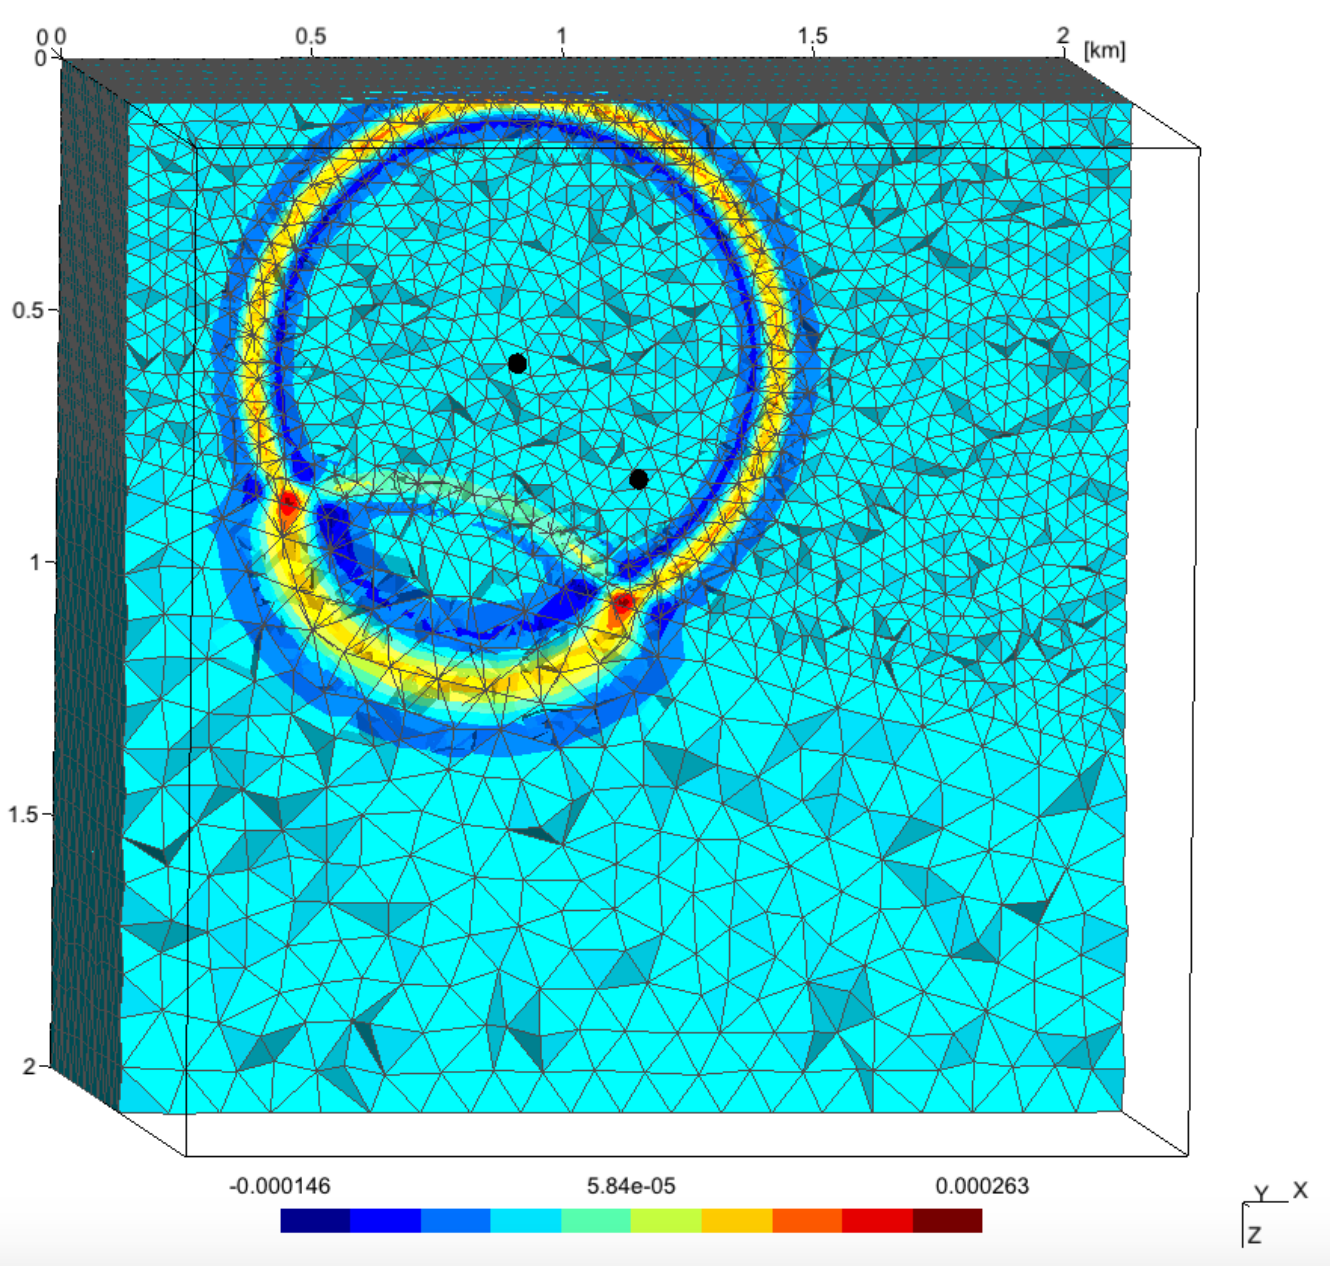
\includegraphics[width=.95\textwidth]{figs/wave.png}
\caption*{Figure courtesy of Axel Modave.}
}
\only<2>{
\includegraphics[width=.95\textwidth]{figs/wave_N1.eps}
\caption*{\textbf{Fine} linear approximation.}
}
\only<3>{
\includegraphics[width=.95\textwidth]{figs/wave_N2.eps}
\caption*{\textbf{Coarse} quadratic approximation.}
}
\only<4>{
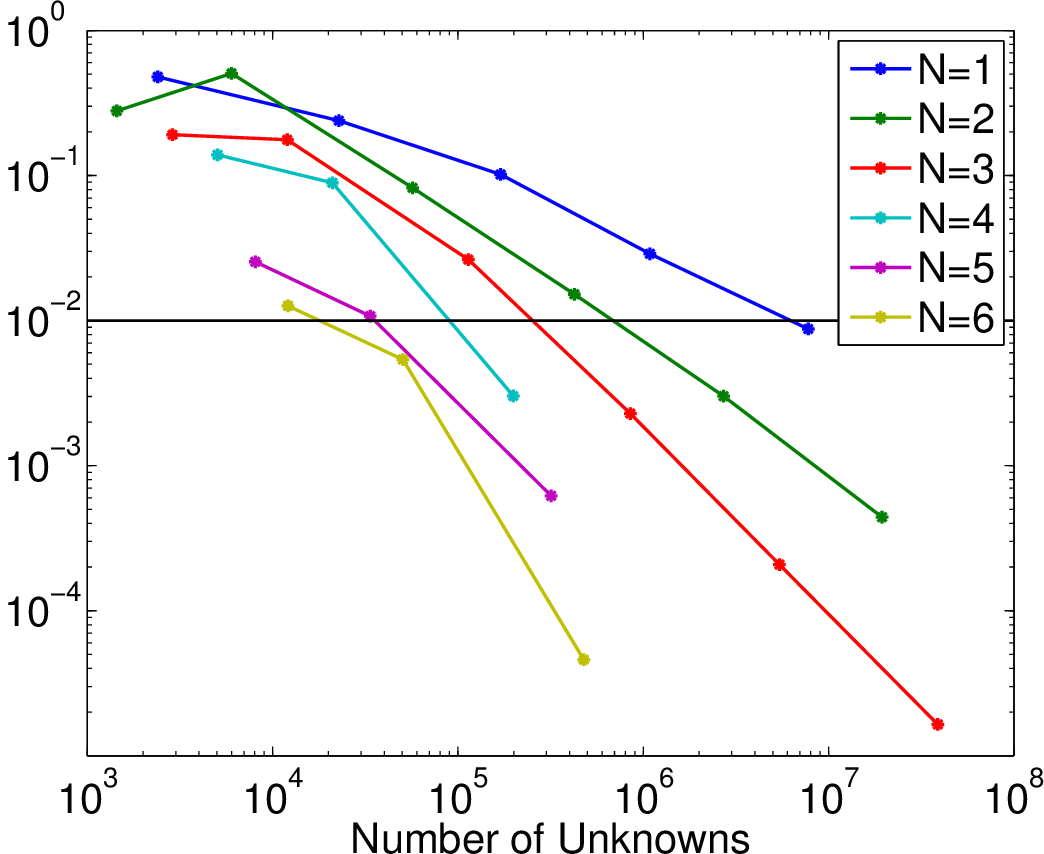
\includegraphics[width=.95\textwidth]{figs/error_v_dofs.png}
\caption*{Max errors vs.\ dofs.}
}
\only<5->{
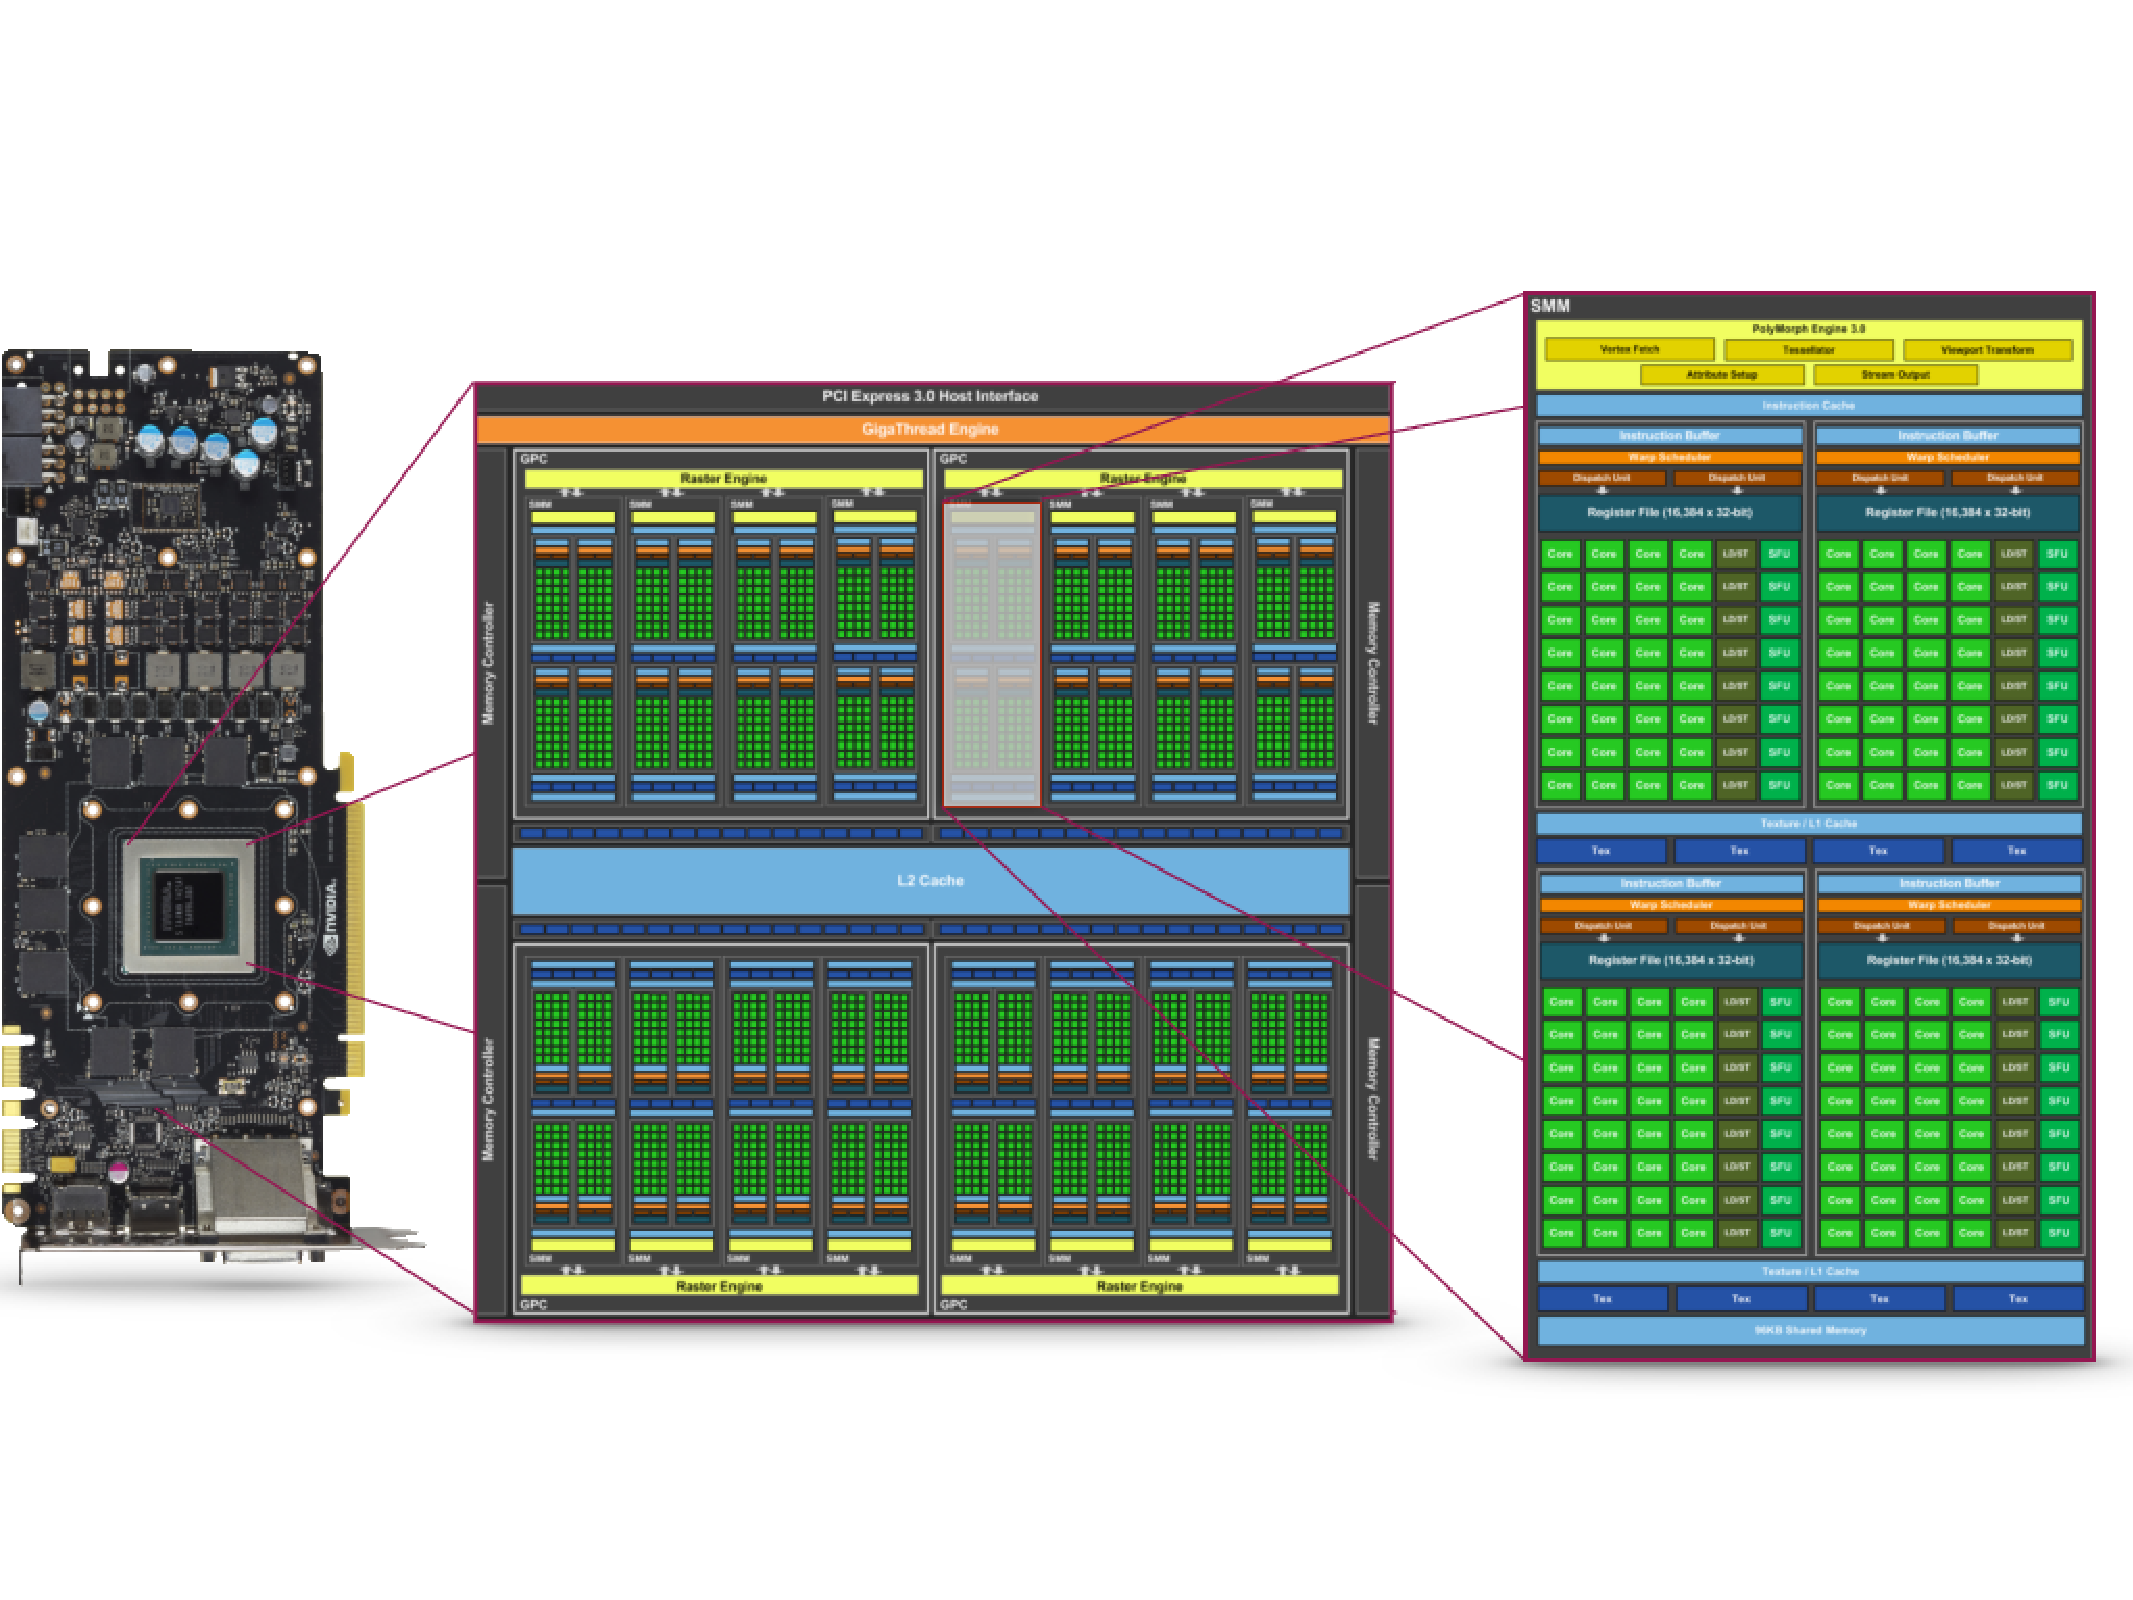
\includegraphics[width=.975\textwidth]{figs/gpu.pdf}
\caption*{Graphics processing units (GPU).}
}
%\caption*{Image courtesy of Axel Modave.}
\end{overlayarea}
\end{figure}
\end{column}
\end{columns}
\vspace{2em}
\uncover<6->{
\begin{center}
\ovalbox{Goal: accuracy \textbf{and} efficiency for heterogeneous media.}
\end{center}
}
}

\frame{
\frametitle{Time-domain nodal DG methods}
%\vspace{-2em}
\begin{columns}
\begin{column}{.55\textwidth}
Assume $u(\bm{x},t) = \sum \bm{u}_j \phi_j(\bm{x})$ on $D^k$
%Given initial condition $u(\mathbf{x},0)$:
\vspace{.5em}
\begin{itemize}
\item<1-> Compute numerical flux at face nodes (\textcolor{red}{non-local}).
\vspace{.25em}
\item<2-> Compute RHS of (\textcolor{blue}{local}) ODE.
\vspace{.25em}
\item<3-> Evolve (\textcolor{blue}{local}) solution using explicit time integration (RK, AB, etc). 
\end{itemize}
\end{column}
\begin{column}{.45\textwidth}
\begin{figure}
\centering
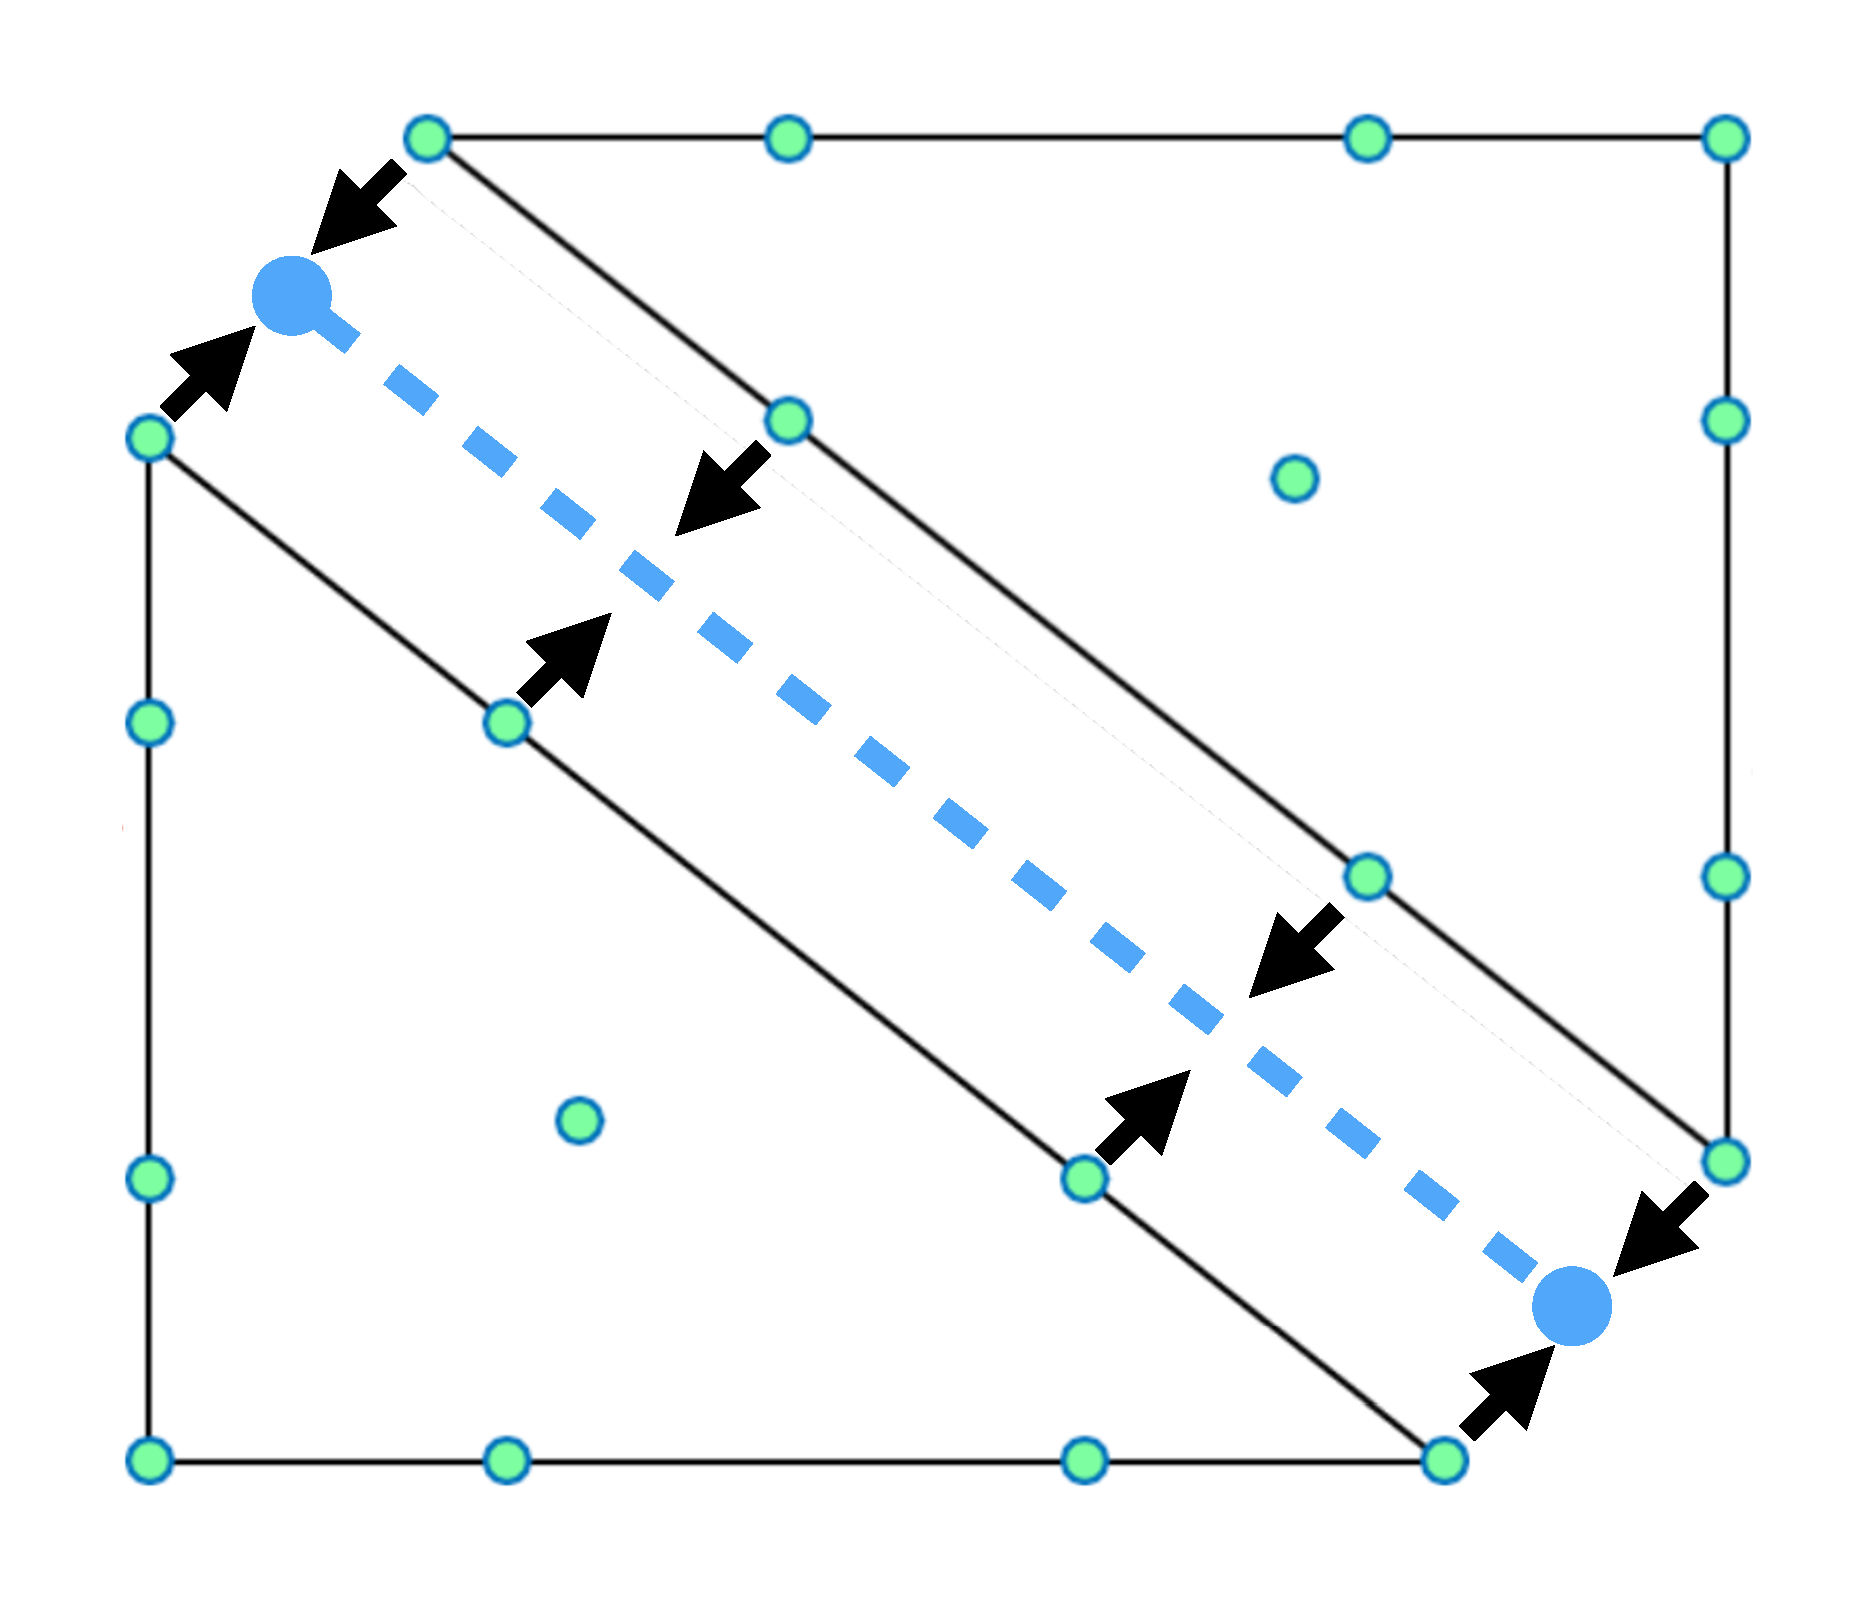
\includegraphics[width=.825\textwidth]{figs/nodal.pdf}
\end{figure}
\end{column}
\end{columns}

\begin{overlayarea}{\textwidth}{.35\textheight}
\begin{columns}
\vspace{.5em}
\begin{column}{.6\textwidth}
\only<1>{
\[
\td{\mathbf{u}}{t} = \mathbf{D}_x \mathbf{u} + \sum_{\text{ faces}}\mathbf{L}_f \LRp{\rm \textcolor{red}{flux}}.%, \qquad \mathbf{L}_f = \mathbf{{M}}^{-1}\mathbf{{M}}_f.
\]
}
\only<2>{
\[
\td{\mathbf{u}}{t} = \underbrace{\mathbf{D}_x \mathbf{u}}_{\text{\textcolor{blue}{Volume kernel}}} + \underbrace{\sum_{\text{ faces}}\mathbf{L}_f \LRp{\rm \textcolor{red}{flux}}}_{\text{\textcolor{blue}{Surface kernel}}}.%, \qquad \mathbf{L}_f = \mathbf{{M}}^{-1}\mathbf{{M}}_f.
\]
}
\only<3->{
\[
\underbrace{\td{\mathbf{u}}{t}}_{\text{\textcolor{blue}{Update kernel}}} = \underbrace{\mathbf{D}_x \mathbf{u}}_{\text{\textcolor{blue}{Volume kernel}}} + \underbrace{\sum_{\text{ faces}}\mathbf{L}_f \LRp{\rm \textcolor{red}{flux}}}_{\text{\textcolor{blue}{Surface kernel}}}.%, \qquad \mathbf{L}_f = \mathbf{{M}}^{-1}\mathbf{{M}}_f.
\]
}
%\uncover<4->{
%\begin{center}
%Well suited to GPUs
%\end{center}
%}
\end{column}
%\vspace{-.5em}
\begin{column}{.4\textwidth}
\begin{gather*}
\bm{M}_{ij} = \int_{D^k} \phi_j(\bm{x})\phi_i(\bm{x})\\
\mathbf{L}_f = \mathbf{{M}}^{-1}\mathbf{{M}}_f.
\end{gather*}
\end{column}
\end{columns}
\end{overlayarea}

}



\section{Weight-adjusted DG (WADG): arbitrary heterogeneous media}

\begin{frame}[noframenumbering]
  \frametitle{Outline}
\only<1>{
 \tableofcontents
}
\only<2>{
 \tableofcontents[currentsection]
}
\end{frame}

\frame{
\frametitle{High order approximation of media and geometry}
\setcounter{subfigure}{0}
\vspace{-1.5em}
\begin{figure}
\subfloat[Mesh and exact $c^2$]{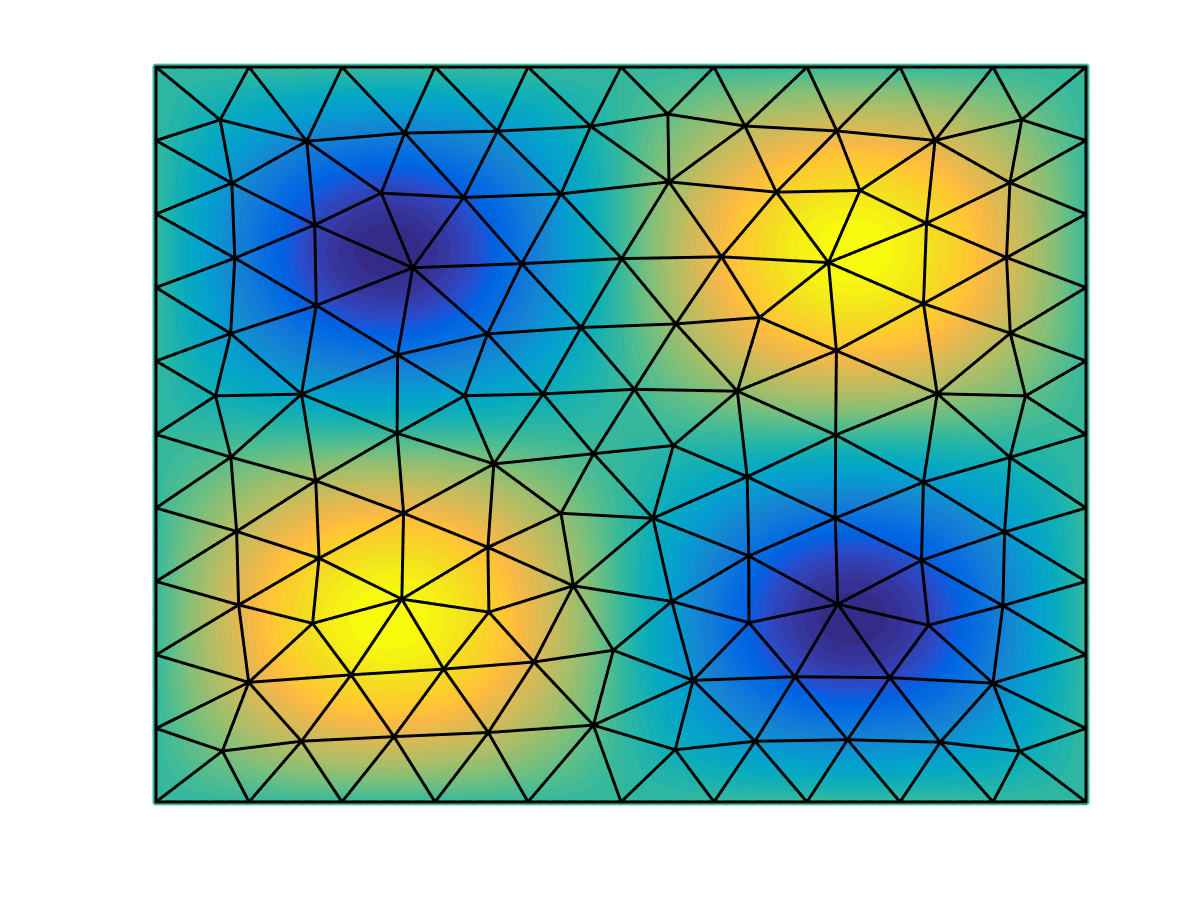
\includegraphics[width=.3175\textwidth]{figs/c2WADG.png}}
%\hspace{.1em}
\subfloat[Piecewise const.\ $c^2$]{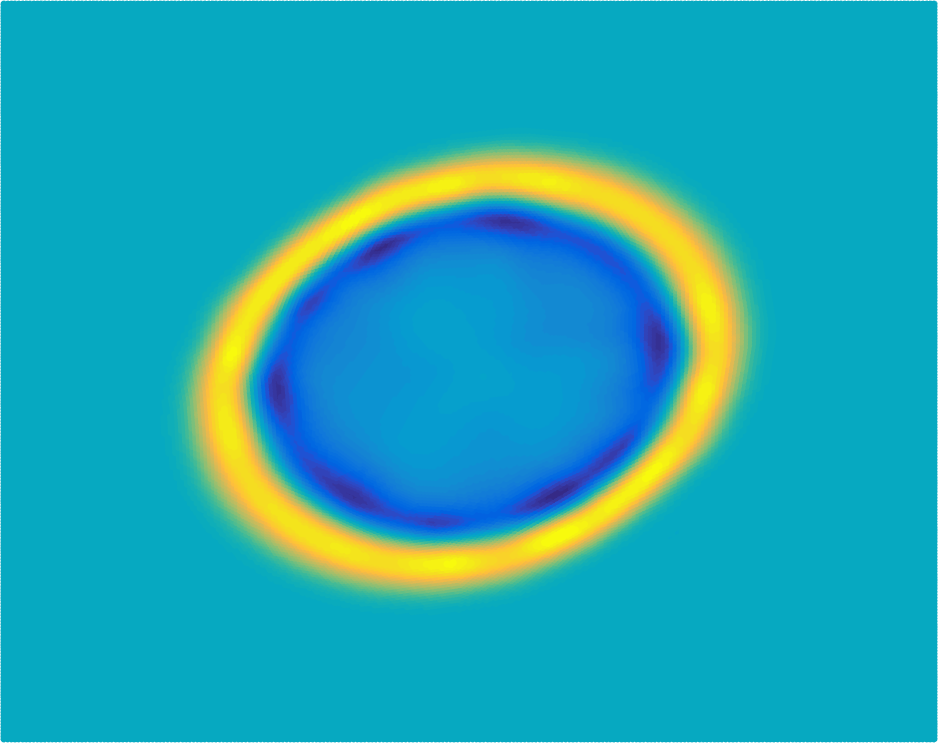
\includegraphics[width=.28\textwidth]{figs/p0WADG.png}}
\hspace{.25em}
\subfloat[High order $c^2$]{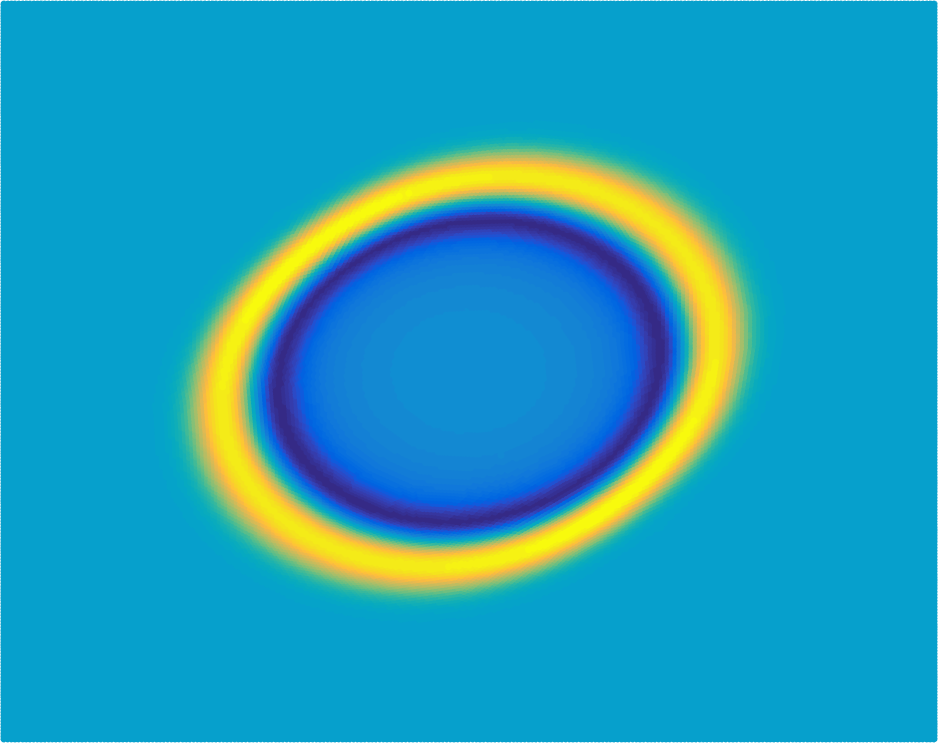
\includegraphics[width=.28\textwidth]{figs/pNWADG.png}}
\end{figure}
%\vspace{-.5em}
\begin{itemize}
\item %Acoustic wave equation: 
Piecewise constant wavespeed $c^2$: efficient, but spurious reflections.
\begin{align*}
\frac{1}{c^2(\bm{x})}\pd{p}{t}{} + \Grad\cdot \bm{u} = 0, \qquad \pd{\bm{u}}{t}{} + \Grad p = 0.
\end{align*}
\item High order wavespeeds: weighted mass matrices. Stable, but requires pre-computation/storage of inverses or factorizations!
\[
\bm{M}_{1/c^2}\td{\bm{p}}{t} = \bm{A}_h\bm{U}, \qquad \LRp{\bm{M}_{1/c^2}}_{ij} = \int_{D^k}\frac{1}{c^2(\bm{x})} \phi_j(\bm{x})\phi_i(\bm{x}).
\]
\end{itemize}
}


%\frame{
%\frametitle{Energy stable discontinuous Galerkin formulations}
%\begin{itemize}
%\item Model problem: acoustic wave equation (pressure-velocity system)
%\begin{align*}
%\frac{1}{c^2(\bm{x})}\pd{p}{t}{} = \Div \bm{u}, \qquad \pd{\bm{u}}{t}{} = \Grad p
%\end{align*}
%\item Local formulation 
%\begin{align*}
%\int_{D^k}\frac{1}{c^2(\bm{x})}\pd{p}{t}{} q &= \int_{D^k} \Div \bm{u} q  + \frac{1}{2}\int_{\partial D^k} \LRp{\jump{\bm{u}}\cdot{\bm{n}} + \tau_p\jump{p}} q\\
%\int_{D^k}\pd{\bm{u}}{t}{} \bm{v} &= \int_{D^k} \Grad p \cdot \bm{v} + \frac{1}{2}\int_{\partial D^k} \LRp{\jump{p} + \tau_u\jump{\bm{u}}\cdot\bm{n}} \bm{v}
%\end{align*}
%\item High order accuracy, semi-discrete energy stability
%\[
%\pd{}{t}{}\LRp{\sum_{k} \int_{D^k} \frac{p^2}{c^2(\bm{x})} + \LRb{\bm{u}}^2} = -\sum_k\int_{\partial D^k} \tau_p\jump{p}^2 +  \tau_u\jump{\bm{u}\cdot\bm{n}}^2 \leq 0.
%\]
%\end{itemize}
%}

%\frame{
%\frametitle{Weighted mass matrices}
%\begin{itemize}
%\item Spatially varying weights appear in DG mass matrices
%\[
%\only<1,5>{\int_{D^k}{\frac{1}{c^2}}\pd{p}{t}{} q = \text{pressure RHS}, \qquad \int_{D^k}\pd{\bm{u}}{t}{} \bm{v} = \text{velocity RHS}}
%\only<2>{\int_{\note{\widehat{D}}}{\frac{1}{c^2}}\pd{p}{t}{} q {J} = \text{pressure RHS}, \qquad \int_{\note{\widehat{D}}}\pd{\bm{u}}{t}{} \bm{v} {J} = \text{velocity RHS}}
%\only<3>{\int_{\widehat{D}}{\frac{1}{c^2}}\pd{p}{t}{} q \note{J} =  \text{pressure RHS}, \qquad \int_{\widehat{D}}\pd{\bm{u}}{t}{} \bm{v} \note{J} = \text{velocity RHS}}
%\only<4>{\int_{\widehat{D}}\note{\frac{1}{c^2}}\pd{p}{t}{} q \note{J} =  \text{pressure RHS}, \qquad \int_{\widehat{D}}\pd{\bm{u}}{t}{} \bm{v} \note{J} = \text{velocity RHS}}
%\]
%\item \only<1-2,4->{Curvilinear}\only<3>{\textcolor{red}{Curvilinear}} meshes and wave propagation in \only<1-3,5>{heterogeneous media}\only<4>{\textcolor{red}{heterogeneous media}} 
%\begin{overlayarea}{\textwidth}{.25\textheight}
%\vspace{-1.25em}
%\only<1-2,5>{
%\begin{align*}
%\LRp{\bm{M}_{w}}_{ij} &= \int_{\widehat{D}}\phi_i \phi_j w(x),\\
%\td{}{t}\bm{M}_{w} \bm{u} &= \text{right hand side}.
%\end{align*}
%}
%\only<3>{
%\begin{align*}
%\LRp{\bm{M}_{w}}_{ij} &= \int_{\widehat{D}}\phi_i \phi_j \textcolor{red}{J(x)}, \\
%\td{}{t}\bm{M}_{\textcolor{red}{J}} \bm{u} &= \text{right hand side}.
%\end{align*}
%}
%\only<4>{
%\begin{align*}
%\LRp{\bm{M}_{w}}_{ij} &= \int_{\widehat{D}}\phi_i \phi_j \textcolor{red}{\frac{J}{c^{2}(x)}}, \\
%\td{}{t}\bm{M}_{\textcolor{red}{J/c^2}} \bm{u} &= \text{right hand side}.
%\end{align*}
%}
%\end{overlayarea}
%\item Inherits \textbf{high order accuracy} and \textbf{energy stability} with respect to a weighted $L^2$ norm, but requires $\bm{M}_w^{-1}$ explicitly \only<1-4>{over each element}\only<5>{\textcolor{red}{over each element}}.
%\vspace{.5em}
%\item On-the-fly assembly + inversion or pre-computation and \only<1-4>{storage}\only<5>{\note{storage}}.
%\end{itemize}
%}

%\frame{
%\frametitle{Inverting weighted mass matrices: storage costs}
%
%\begin{itemize}
%\item Assembling and inverting $\bm{M}_w$ on-the-fly
%\begin{itemize}
%\item High computational complexity w.r.t.\ $N$.
%\item Fine-grain parallelization of solve more difficult.
%\end{itemize}
%\vspace{1em}
%\item Pre-computation and storage of $\bm{M}_w^{-1}$ 
%\begin{itemize}
%\item Increase from $O(N^3)$ to $O(N^6)$ storage per element.
%\end{itemize}
%\end{itemize}
%\vspace{2em}
%Memory costs of DG (\emph{single precision}, one field, 3D tets, 1M elements):
%\begin{table}
%\centering                                                                                   
%\begin{tabular}{| c | c | c | c | c |}
%\hline
%Order $N$ & $N=1$ & $N=3$ & $N=5$ & $N=7$ \\
%\hline
%Block matrix $M^{-1}$ & .298 GB  & \textcolor{red}{3.2 GB}  & \textcolor{red}{25.08 GB} & \textcolor{red}{115.2 GB} \\
%\hline
%Solution dofs & .075 GB  & .16 GB  & .448 GB & .96 GB \\
%\hline 
%\end{tabular}
%\label{table:cost}
%\end{table}
%%\begin{center}
%%Large storage costs at high order: need mass matrix inverses if $w = w(\bm{x})$.  \textcolor{red}{Inefficient for accelerator architectures!}
%%\end{center}
%}

%\frame{
%\frametitle{Weight-adjusted DG: convergence and implementation}
%\begin{itemize}
%\item \textcolor{red}{Weight-adjusted DG (WADG)}: energy stable approximation of weighted mass matrix  
%\[
%\bm{M}_{w}\td{\bm{U}}{t} \approx \textcolor{red}{{\bm{M}} \LRp{{\bm{M}}_{1/w}}^{-1} {\bm{M}}} \td{\bm{U}}{t} = \text{right hand side}.
%\]
%\item WADG \textit{a-priori} estimates: optimal weighted projection estimate shows \textbf{high order accuracy}:
%\begin{align*}
%&\nor{u - P_w u}_{L^2} \leq C h^{N+1}  \nor{w}_{W^{N+1,\infty}} \nor{\frac{\sqrt{J}}{w}}_{L^{\infty}} \nor{u}_{W^{N+1,2}}.
%\end{align*}
%\item Bypasses inverse of weighted matrix $\LRp{\bm{M}_{w}}^{-1}$ 
%\[
%\LRp{{\bm{M}} \LRp{{\bm{M}}_{1/w}}^{-1}{\bm{M}}}^{-1} = {\bm{M}}^{-1} {{\bm{M}}}_{1/w} {\bm{M}}^{-1}.
%\]
%\end{itemize}
%}

\frame{
\frametitle{Weight-adjusted DG: stable, accurate, non-invasive}
\begin{itemize}
\item \textcolor{red}{Weight-adjusted DG (WADG)}: energy stable approx.\ of $\bm{M}_{1/c^2}$
\[
\bm{M}_{1/c^2}\td{\bm{p}}{t} \approx \textcolor{red}{{\bm{M}} \LRp{{\bm{M}}_{c^2}}^{-1} {\bm{M}}} \td{\bm{p}}{t} = \bm{A}_h\bm{U}.%\text{right hand side}.
\]
%\item Bypasses inverse of weighted matrix $\LRp{\bm{M}_{1/c^2}}^{-1}$ 
%\[
%\LRp{{\bm{M}} \LRp{{\bm{M}}_{c^2}}^{-1}{\bm{M}}}^{-1} = {\bm{M}}^{-1} {{\bm{M}}}_{c^2} {\bm{M}}^{-1}.
%\]
%\vspace{.01em}
\item New evaluation reuses implementation for constant wavespeed
\begin{align*}
%{\bm{M}} \LRp{{\bm{M}}_{c^2}}^{-1} {\bm{M}} \td{\bm{U}}{t} &= \bm{A}_h \bm{U} \\
%\rightarrow 
\td{\bm{p}}{t} &= \underbrace{{\bm{M}}^{-1}\LRp{{\bm{M}}_{c^2}}}_{\text{modified update}}  \quad \underbrace{\bm{M}^{-1}\bm{A}_h \bm{U} }_{\text{constant wavespeed RHS}}
\end{align*}
%\vspace{.01em}
\item Low storage matrix-free application of $\bm{M}^{-1}{\bm{M}}_{c^2}$ using \textbf{quadrature}-based interpolation and $L^2$ projection matrices $\bm{V}_q,\bm{P}_q$.  
\[
\LRp{\bm{M}}^{-1} {\bm{M}}_{c^2}\text{RHS} = \underbrace{{\bm{M}}^{-1} \bm{V}_q^T W}_{\bm{P}_q} {\rm diag}\LRp{c^2} \bm{V}_q \LRp{\text{RHS}}.
\]

\end{itemize}
\let\thefootnote\relax\footnotetext{\tiny Chan, Hewett, Warburton.\ 2016.  {Weight-adjusted DG methods: wave propagation in heterogeneous media} (SISC).}

}


\frame{
\frametitle{WADG: nearly identical to using $\bm{M}^{-1}_{1/c^2}$}
\setcounter{subfigure}{0}
\vspace{-1em}
\begin{figure}
\centering
\only<1>{
\subfloat[$c^2(x,y)$]{
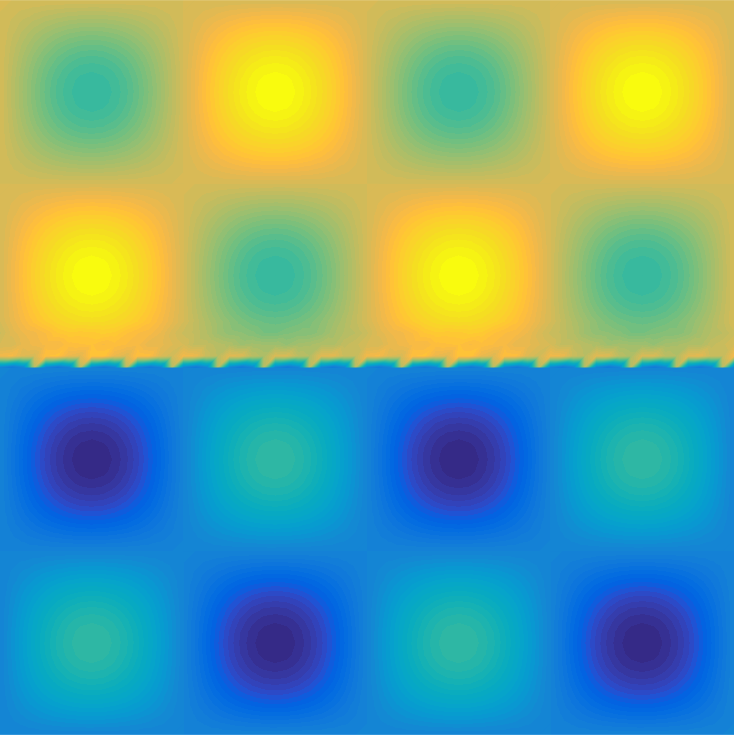
\includegraphics[width=.32\textwidth]{figs/cfun.png}
}
\hspace{1em}
\subfloat[Standard DG]{
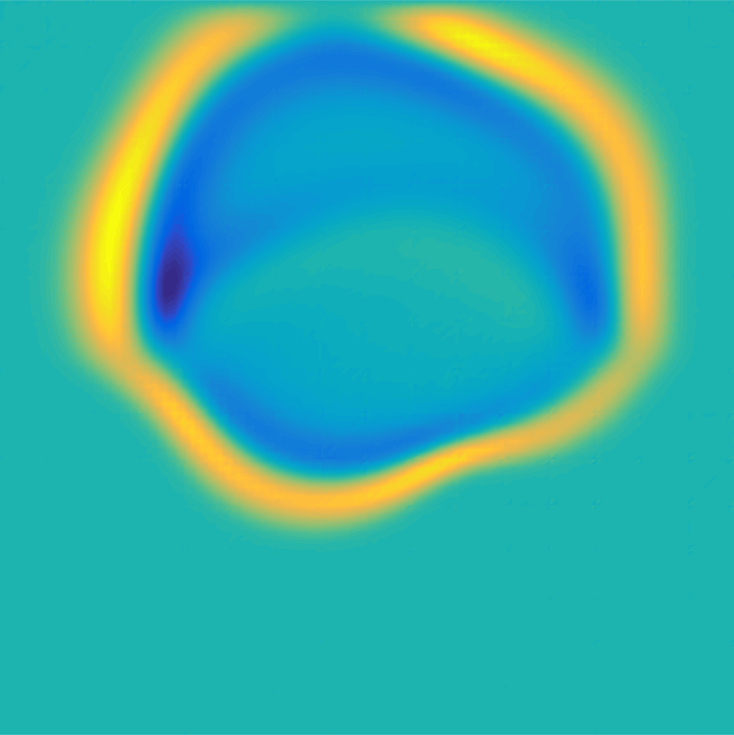
\includegraphics[width=.32\textwidth]{figs/cmass_wave.png}
}}
\only<2>{
\subfloat[$c^2(x,y)$]{
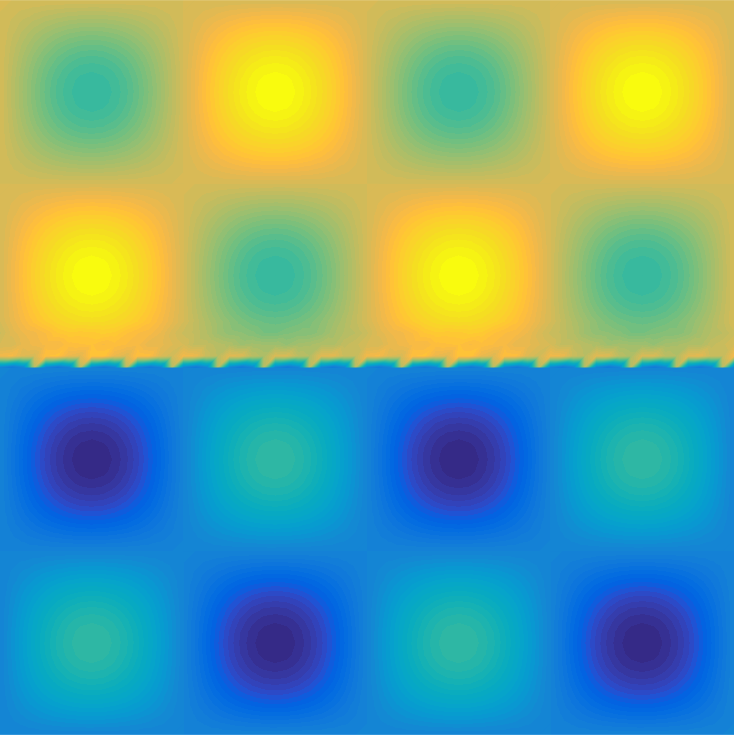
\includegraphics[width=.32\textwidth]{figs/cfun.png}
}
\hspace{1em}
\subfloat[Weighted-adjusted DG]{
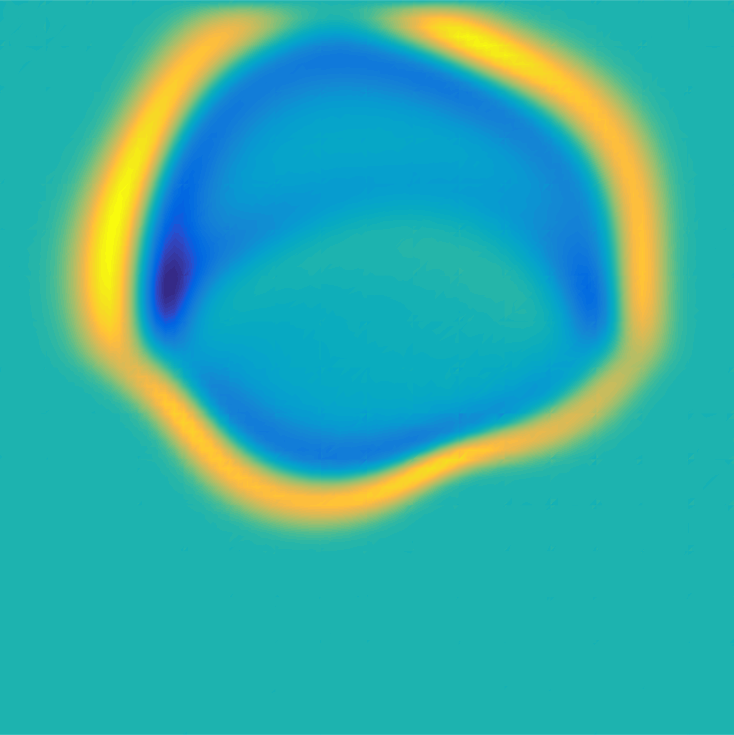
\includegraphics[width=.32\textwidth]{figs/cproj_wave.png}
}}
\caption{Standard vs.\ weight-adjusted DG with spatially varying $c^2$.  }
\end{figure}
\vspace{-.5em}
\begin{itemize}
\item $L^2$ error is $O(h^{N+1})$; standard DG and WADG difference is $O(h^{N+2})$.
\item Can generalize to matrix weights (elastic wave propagation).
\end{itemize}

\let\thefootnote\relax\footnotetext{\tiny Chan 2017.  Weight-adjusted DG methods: matrix-valued weights and elastic wave prop.\ in heterogeneous media (IJNME).}
}

%\frame{
%\frametitle{Matrix-valued weights and elastic wave propagation}
%\begin{itemize}
%\item Symmetric velocity-stress form of linear elasticity ($\bm{A}_i$ constant)
%\begin{align*}
%\rho\pd{\bm{v}}{t}{} = \sum_{i=1}^d \bm{A}_i^T \pd{\bm{\sigma}}{\bm{x}_i}{}, \qquad \bm{C}^{-1}\pd{\bm{\sigma}}{t}{} = \sum_{i=1}^d \bm{A}_i \pd{\bm{v}}{\bm{x}_i}{}.
%\end{align*}
%\item DG formulation based on penalty fluxes, matrix-weighted mass matrix
%\[
%{\bm{M}_{\bm{C}^{-1}}} = \LRp{\begin{array}{ccc}
%\bm{M}_{C^{-1}_{11}} & \ldots & \bm{M}_{C^{-1}_{1d}}\\
%\vdots & \ddots & \vdots\\
%\bm{M}_{C^{-1}_{d1}} & \ldots & \bm{M}_{C^{-1}_{dd}}\\
%\end{array}}
%\]
%\item Weight-adjusted approximation for $\bm{C}^{-1}$ decouples each component
%\[
%\bm{M}_{\bm{C}^{-1}}^{-1} \approx \LRp{\bm{I}\otimes \bm{M}^{-1}} \bm{M}_{\bm{C}} \LRp{\bm{I} \otimes\bm{M}^{-1}}.
%\]
%\end{itemize}
%}


%\frame{
%\frametitle{Matrix-weighted WADG: elastic wave propagation}
%\setcounter{subfigure}{0}
%\begin{figure}
%\centering
%\subfloat[Piecewise constant data]{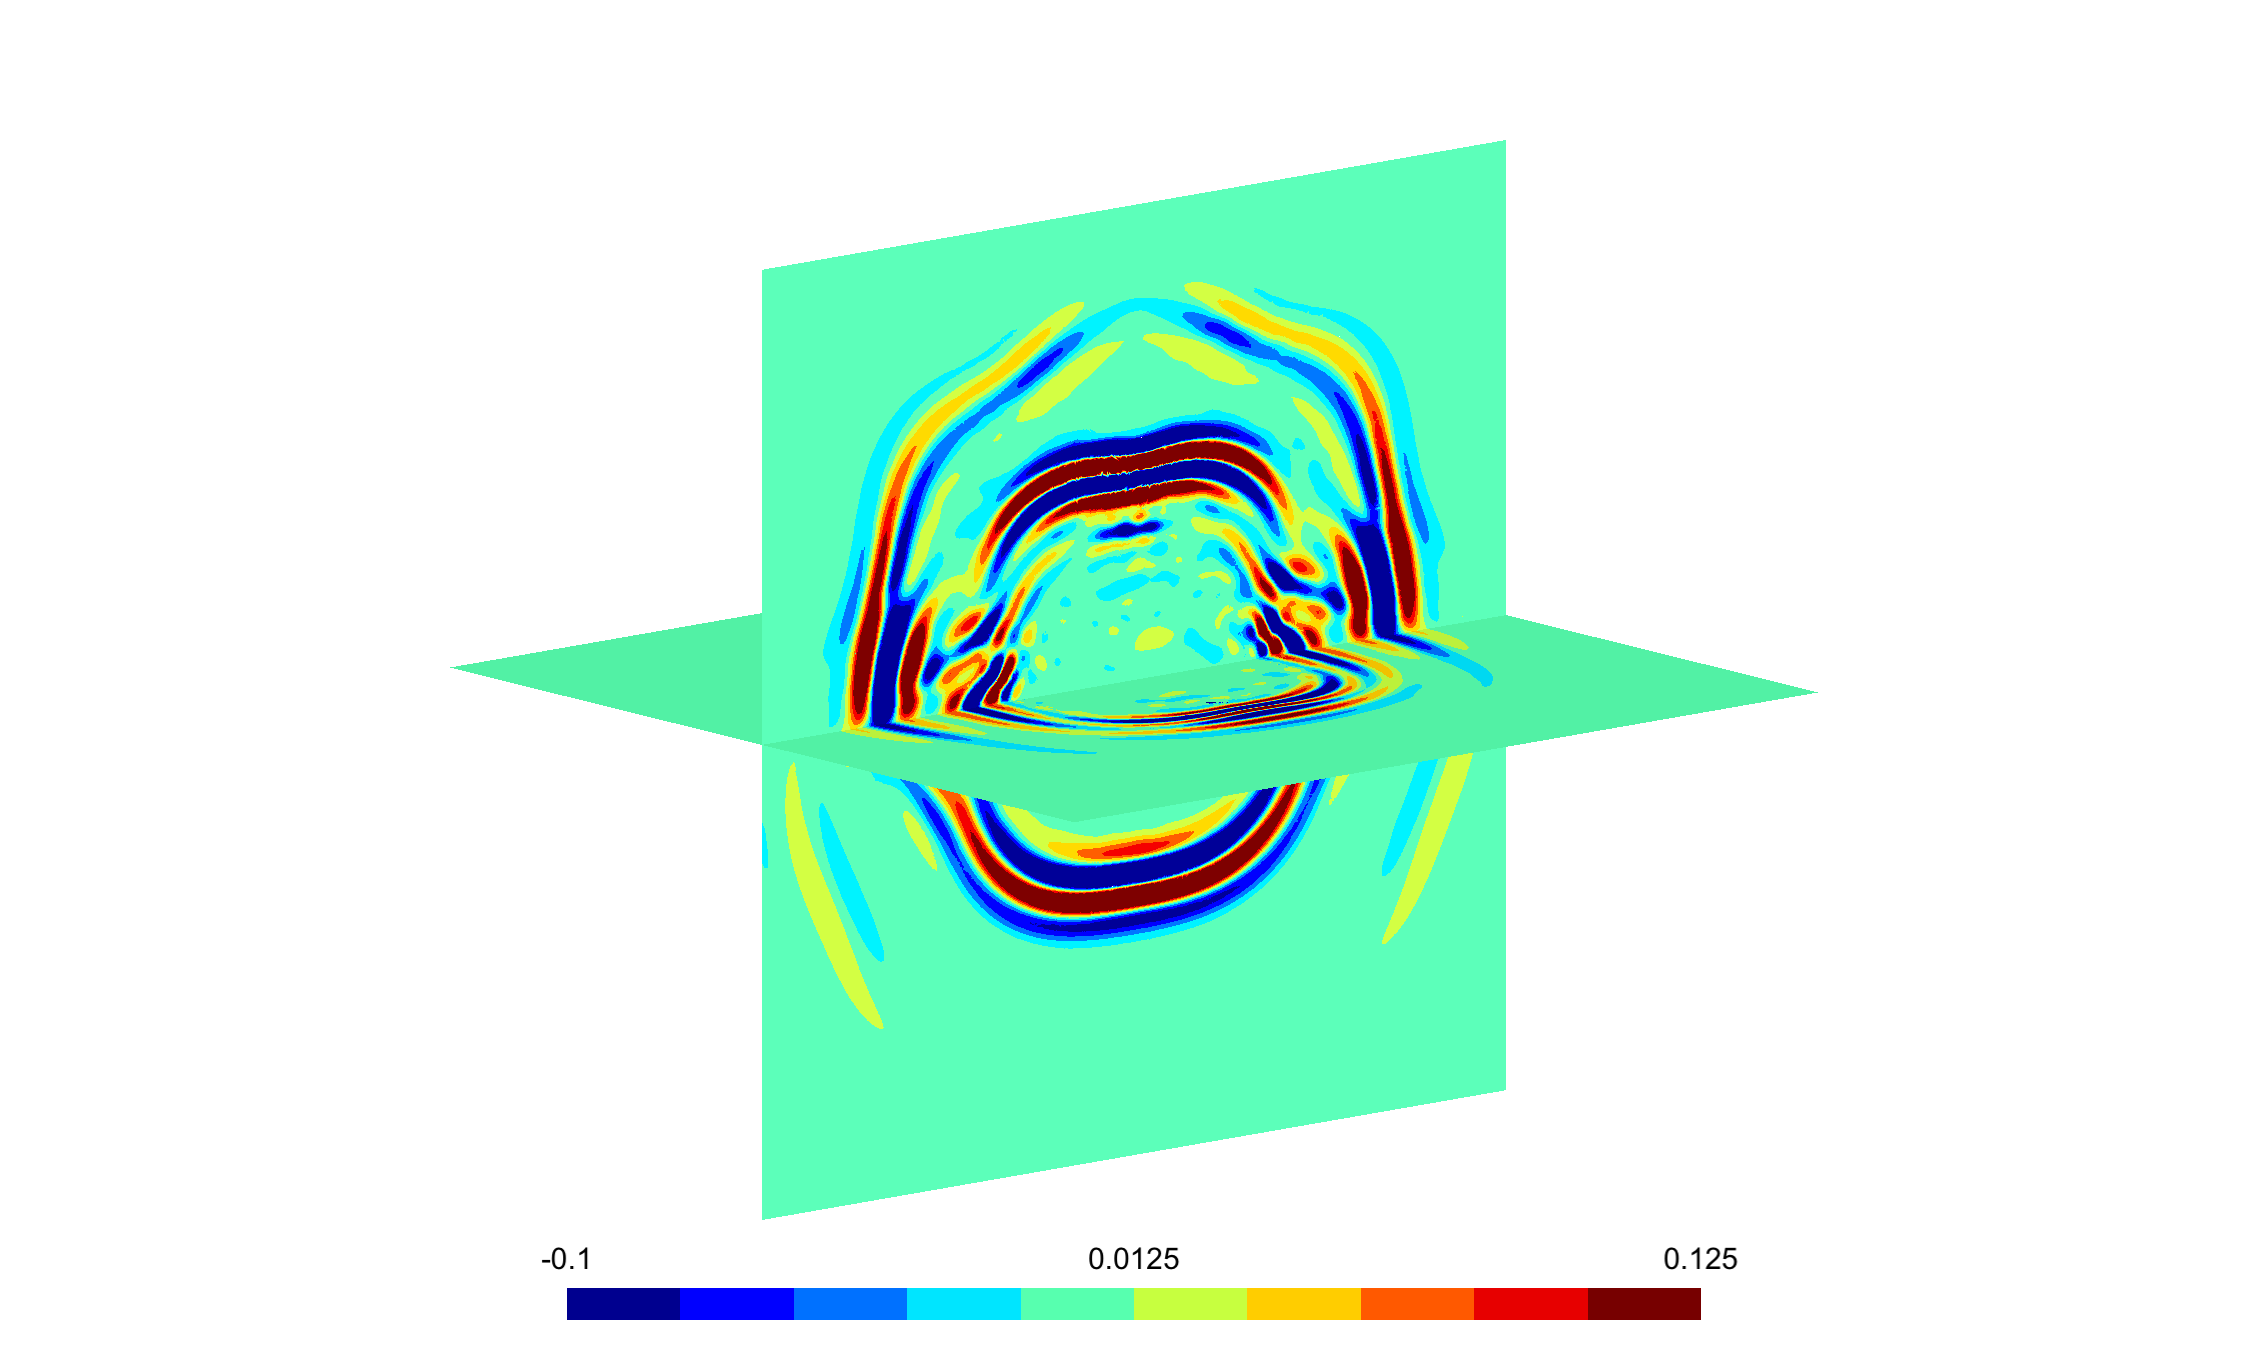
\includegraphics[width=.475\textwidth]{figs/pplanec0.png}}
%\subfloat[High order data]{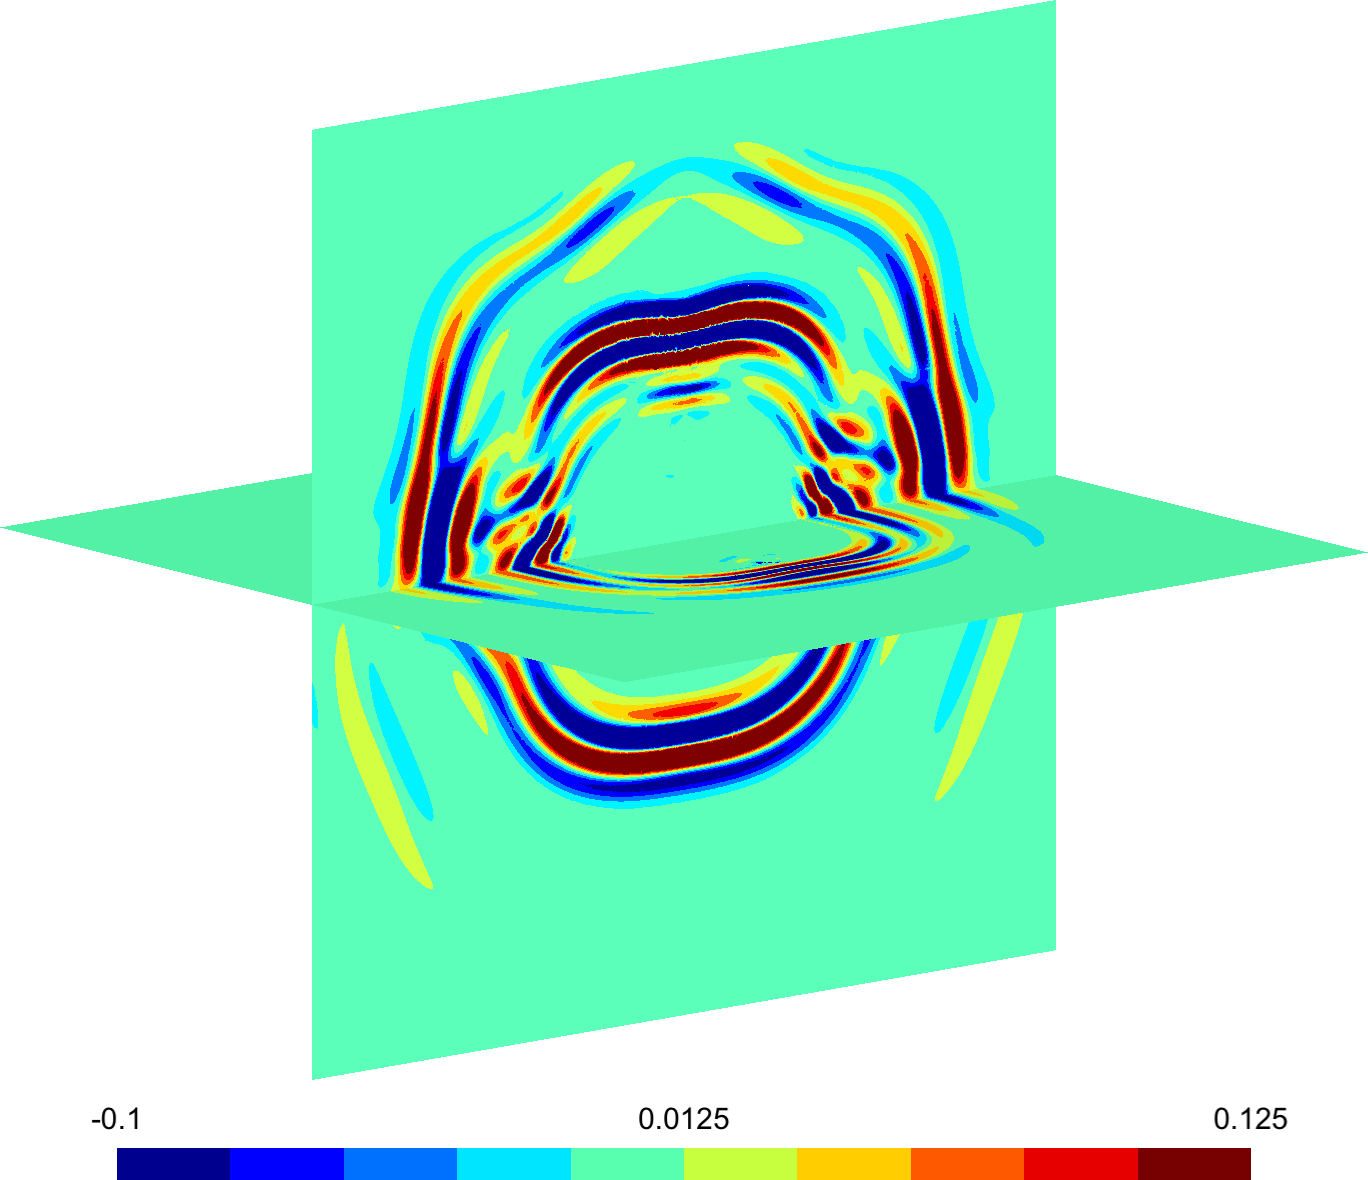
\includegraphics[width=.475\textwidth]{figs/pplanew0.png}}
%\caption{${\rm tr}(\bm{\sigma})$ with $\mu(\bm{x}) = 1+ H(y) + \frac{1}{2}\cos(3\pi x)\cos(3\pi y)\cos(3\pi z)$, $N=5$.}
%\end{figure}
%}

\frame{
\frametitle{WADG: more efficient than storing $\bm{M}^{-1}_{1/c^2}$ on GPUs}

\begin{table}
\centering
\begin{tabular}{|c||c|c|c|c|c|c|c|}
\hline
& $N = 1$ & $N = 2$ & $N = 3$ & $N = 4$ & $N = 5$ & $N = 6$ & $N = 7$\\
\hline
$\bm{M}_{1/c^2}^{-1}$ & .66 & 2.79 & 9.90 &29.4 & 73.9 & 170.5 & 329.4\\
\hline
%WADG & .58 & 1.96 & 6.79 & 22.2 & 56.4 & 129.9 &393\\
WADG & 0.59 &   1.44   & 4.30 &   13.9 &   43.0 & 107.8 &  227.7\\
\hline
Speedup &  1.11 &    1.94 &    2.30 &    2.16 &    1.72 &   1.58 &    1.45\\
\hline
\end{tabular}
\caption*{Time (ns) per element: storing/applying $\bm{M}^{-1}_{1/c^2}$ vs WADG (deg.\ $2N$ quadrature).}
\end{table}

\begin{itemize}
\item Efficiency on GPUs: reduce memory accesses and data movement.
\vspace{.5em}
\item (Tuned) low storage WADG faster than storing and applying $\bm{M}^{-1}_{1/c^2}$!
\end{itemize}
}

%\section{Bernstein-Bezier DG: efficiency for piecewise constant media}
%\frame{
%  \frametitle{Outline}  
%%\only<1>{
%% \tableofcontents
%%}
%%\only<2>{
% \tableofcontents[currentsection]
%%}
%}

\section{Bernstein-Bezier WADG: high order efficiency }


\frame{
%\frametitle{Nodal tetrahedra at high order}
\frametitle{Computational costs at high orders of approximation}

%\begin{itemize}
%%\item Hexahedra: tensor product structure $\rightarrow$ $O(N^4)$ vs $O(N^6)$ local cost.
%%\item How do (naively implemented) nodal tetrahedra behave at high order?
%\item 
%\end{itemize}
%\vspace{-.25em}
\begin{center}
Problem: WADG at high orders becomes \textbf{expensive}!
\end{center}
\vspace{-.5em}
\begin{columns}
\begin{column}{.55\textwidth}
\begin{figure}
\centering
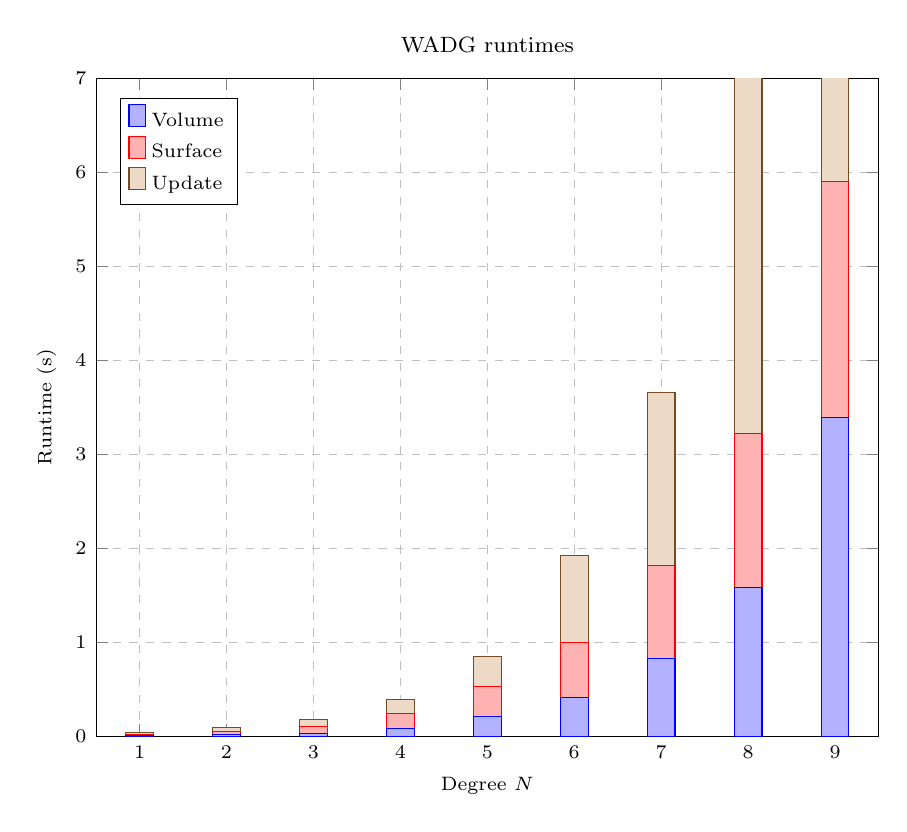
\begin{tikzpicture}
\begin{axis}[
	width=.95\textwidth,
	legend cell align=left,
	%title={Runtime (NPT nodal)},
	title={WADG runtimes},
	xlabel={Degree $N$},
	ylabel={Runtime (s)},
	xmin=.5, xmax=9.5,
	ymin=0,ymax=7,
	ybar stacked,
%	nodes near coords,
	%xmin=.5, xmax=9.5,
	xtick={1,2,3,4,5,6,7,8,9},
	legend pos=north west,
	xmajorgrids=true,
	ymajorgrids=true,
	grid style=dashed,
] 
%nodal runtimes
\addplot coordinates{(1,0.00529)(2,0.0135)(3,0.0302)(4,0.0854)(5,0.206)(6,0.41)(7,0.829)(8,1.58)(9,3.39)};
\addplot coordinates{(1,0.0121)(2,0.0403)(3,0.0722)(4,0.158)(5,0.322)(6,0.587)(7,0.987)(8,1.64)(9,2.51)};
%\addplot coordinates{(1,0.00289997)(2,0.00707789)(3,0.0211354)(4,0.0683213)(5,0.211452)(6,0.530006)(7,1.11929)};
%\addplot coordinates{(1,0.0242951)(2,0.0510198)(3,0.0916193)(4,0.183583)(5,0.397246)(6,1.15212)(7,2.30179)(8,14.2639)};
\addplot coordinates{(1,0.0194361)(2,0.0408158)(3,0.0732955)(4,0.146866)(5,0.317797)(6,0.921698)(7,1.84143)(8,11.4111)(9,21)};


%\addplot coordinates{(1,0.009394)(2,0.025607)(3,0.046205)(4,0.080841)(5,0.142045)(6,0.19389)(7,0.27628)(8,0.381)(9,0.5088)};
%\addplot coordinates{(1,0.026784)(2,0.079407)(3,0.148605)(4,0.324241)(5,0.670045)(6,1.19089)(7,2.09228)(8,3.601)(9,6.4088)};

\legend{Volume, Surface, Update}
%\legend{Volume, Surface}
\end{axis}
\end{tikzpicture}
%\caption*{Per-kernel runtimes for tetrahedra with nodal basis.  Runtimes are recorded for ten RK4 timesteps on a mesh of 98304 elements.}
%\caption*{DG runtimes for 50 timesteps and 98304 elements.}
\caption*{\scriptsize WADG runtimes for 50 timesteps, 98304 elements.}
\end{figure}
\end{column}
\begin{column}{.45\textwidth}
\vspace{-2em}
\begin{itemize}
\item Large \textbf{dense} matrices: $O(N^6)$ work per tet.
\vspace{1em}
\item High orders usually use tensor-product elements: $O(N^{4})$ vs $O(N^{6})$ cost, but less geometric flexibility.
\vspace{1em}
\item Idea: choose basis such that matrices are \textbf{sparse}.
%\item $O(N^{4})$ vs $O(N^6)$ cost, but less geometric flexibility.
\end{itemize}
\end{column}
\end{columns}
}

\frame{
\frametitle{BBDG: Bernstein-Bezier DG methods}
\setcounter{subfigure}{0}

\begin{itemize}
%\item Hexahedral meshes: $O(N^4)$ with tensor product.
\item<1-> Nodal DG: $O(N^6)$ cost in 3D vs $O(N^3)$ degrees of freedom.
\item<2-> Switch to Bernstein basis: sparse and structured matrices.%, $(d+1)$ non-zeros per row.
\item<4-> Optimal $O(N^3)$ application of differentiation and lifting matrices.
\end{itemize}

\begin{figure}
\begin{overlayarea}{.875\textwidth}{.5\textheight}
\only<1>{
\centering
\subfloat{\includegraphics[width=.275\textwidth]{figs/nodal1D.eps}}
%\hspace{.125em}
\subfloat{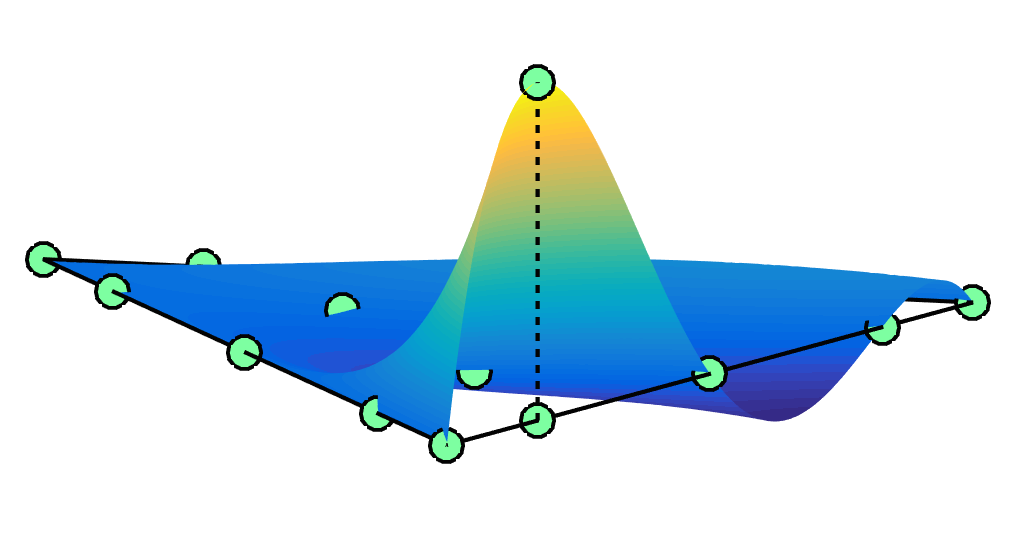
\includegraphics[width=.375\textwidth]{figs/nodal2D.png}}
%\hspace{.125em}
\subfloat{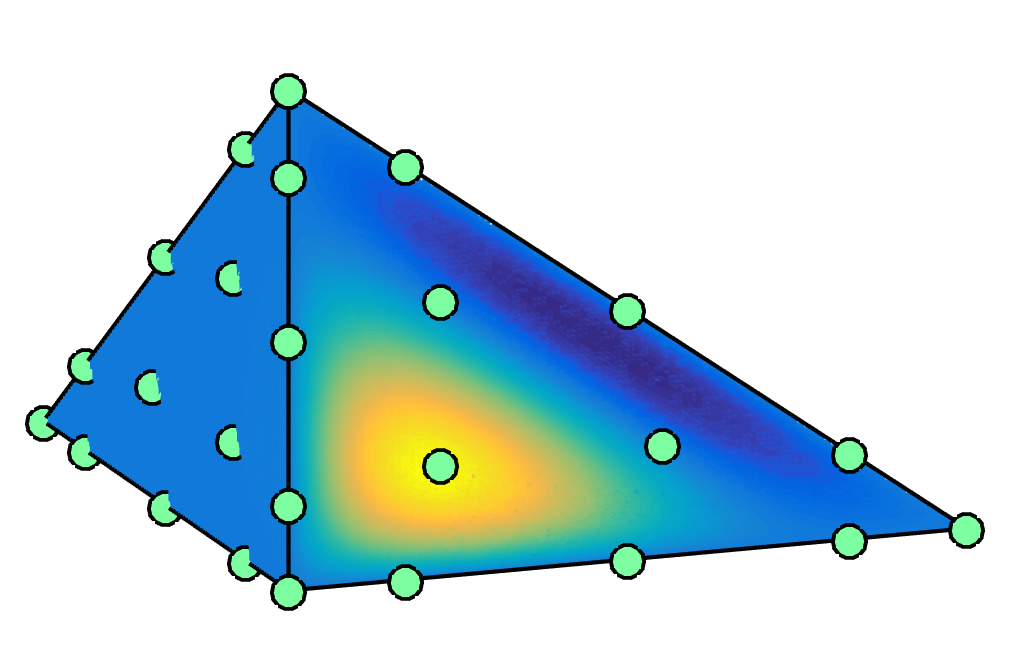
\includegraphics[width=.375\textwidth]{figs/nodal3D.png}}
\vspace{1em}
\caption*{Nodal bases in one, two, and three dimensions.}
}
\only<2>{
\centering
\subfloat{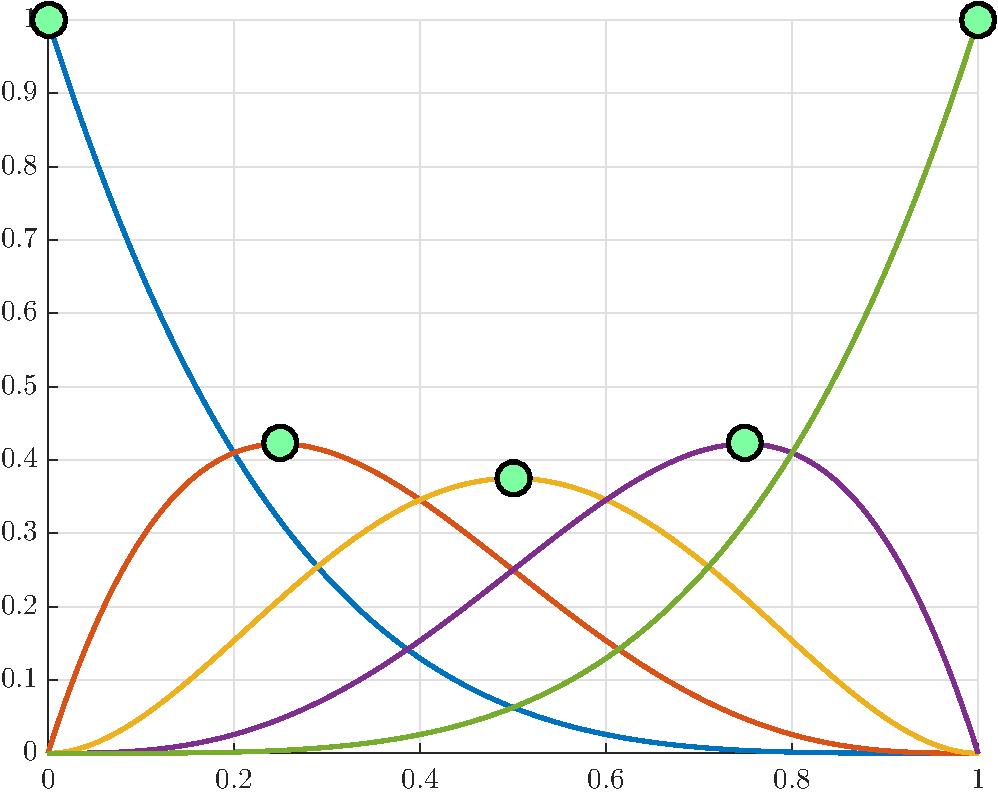
\includegraphics[width=.275\textwidth]{figs/bern1D.pdf}}
%\hspace{.125em}
\subfloat{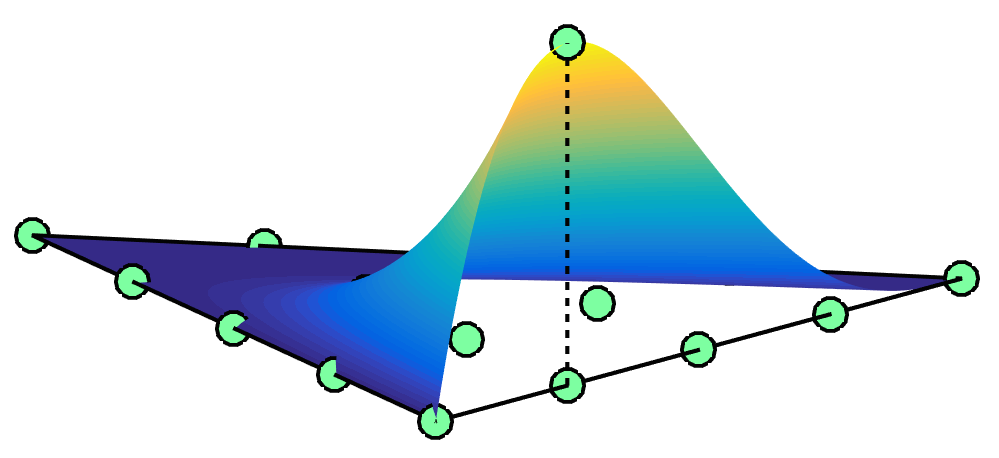
\includegraphics[width=.375\textwidth]{figs/bern2D.png}}
%\hspace{.125em}
\subfloat{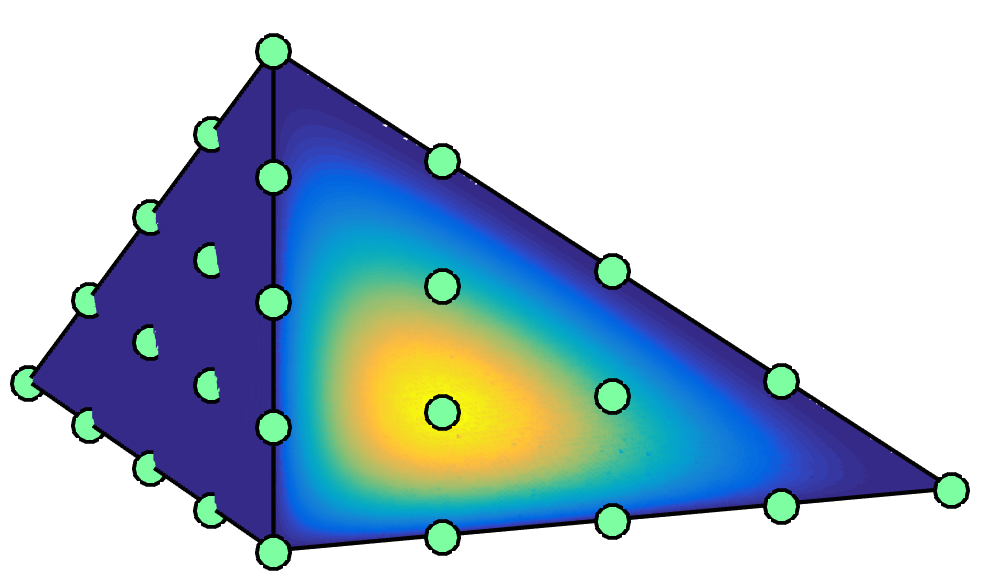
\includegraphics[width=.375\textwidth]{figs/bern3D.png}}
\vspace{1em}
\caption*{Bernstein bases in one, two, and three dimensions.}
}
\only<3>{
\centering
\subfloat{\includegraphics[width=.31\textwidth]{figs/spyD_BB1.png}}
\hspace{.5em}
\subfloat{\includegraphics[width=.31\textwidth]{figs/spyD_BB3.png}}
\hspace{.5em}
\subfloat{\includegraphics[width=.31\textwidth]{figs/spyD_BB4.png}}
%\hspace{3em}
%\subfloat[$\bm{E}_{N-1}^N$]{\includegraphics[height=.425\textheight]{figs/spyE1.eps}}
%\caption{Sparse Bernstein derivative and degree elevation matrices. }
\caption*{Sparse Bernstein differentiation matrices for the reference tetrahedron. }
}
\only<4>{
\centering
\subfloat{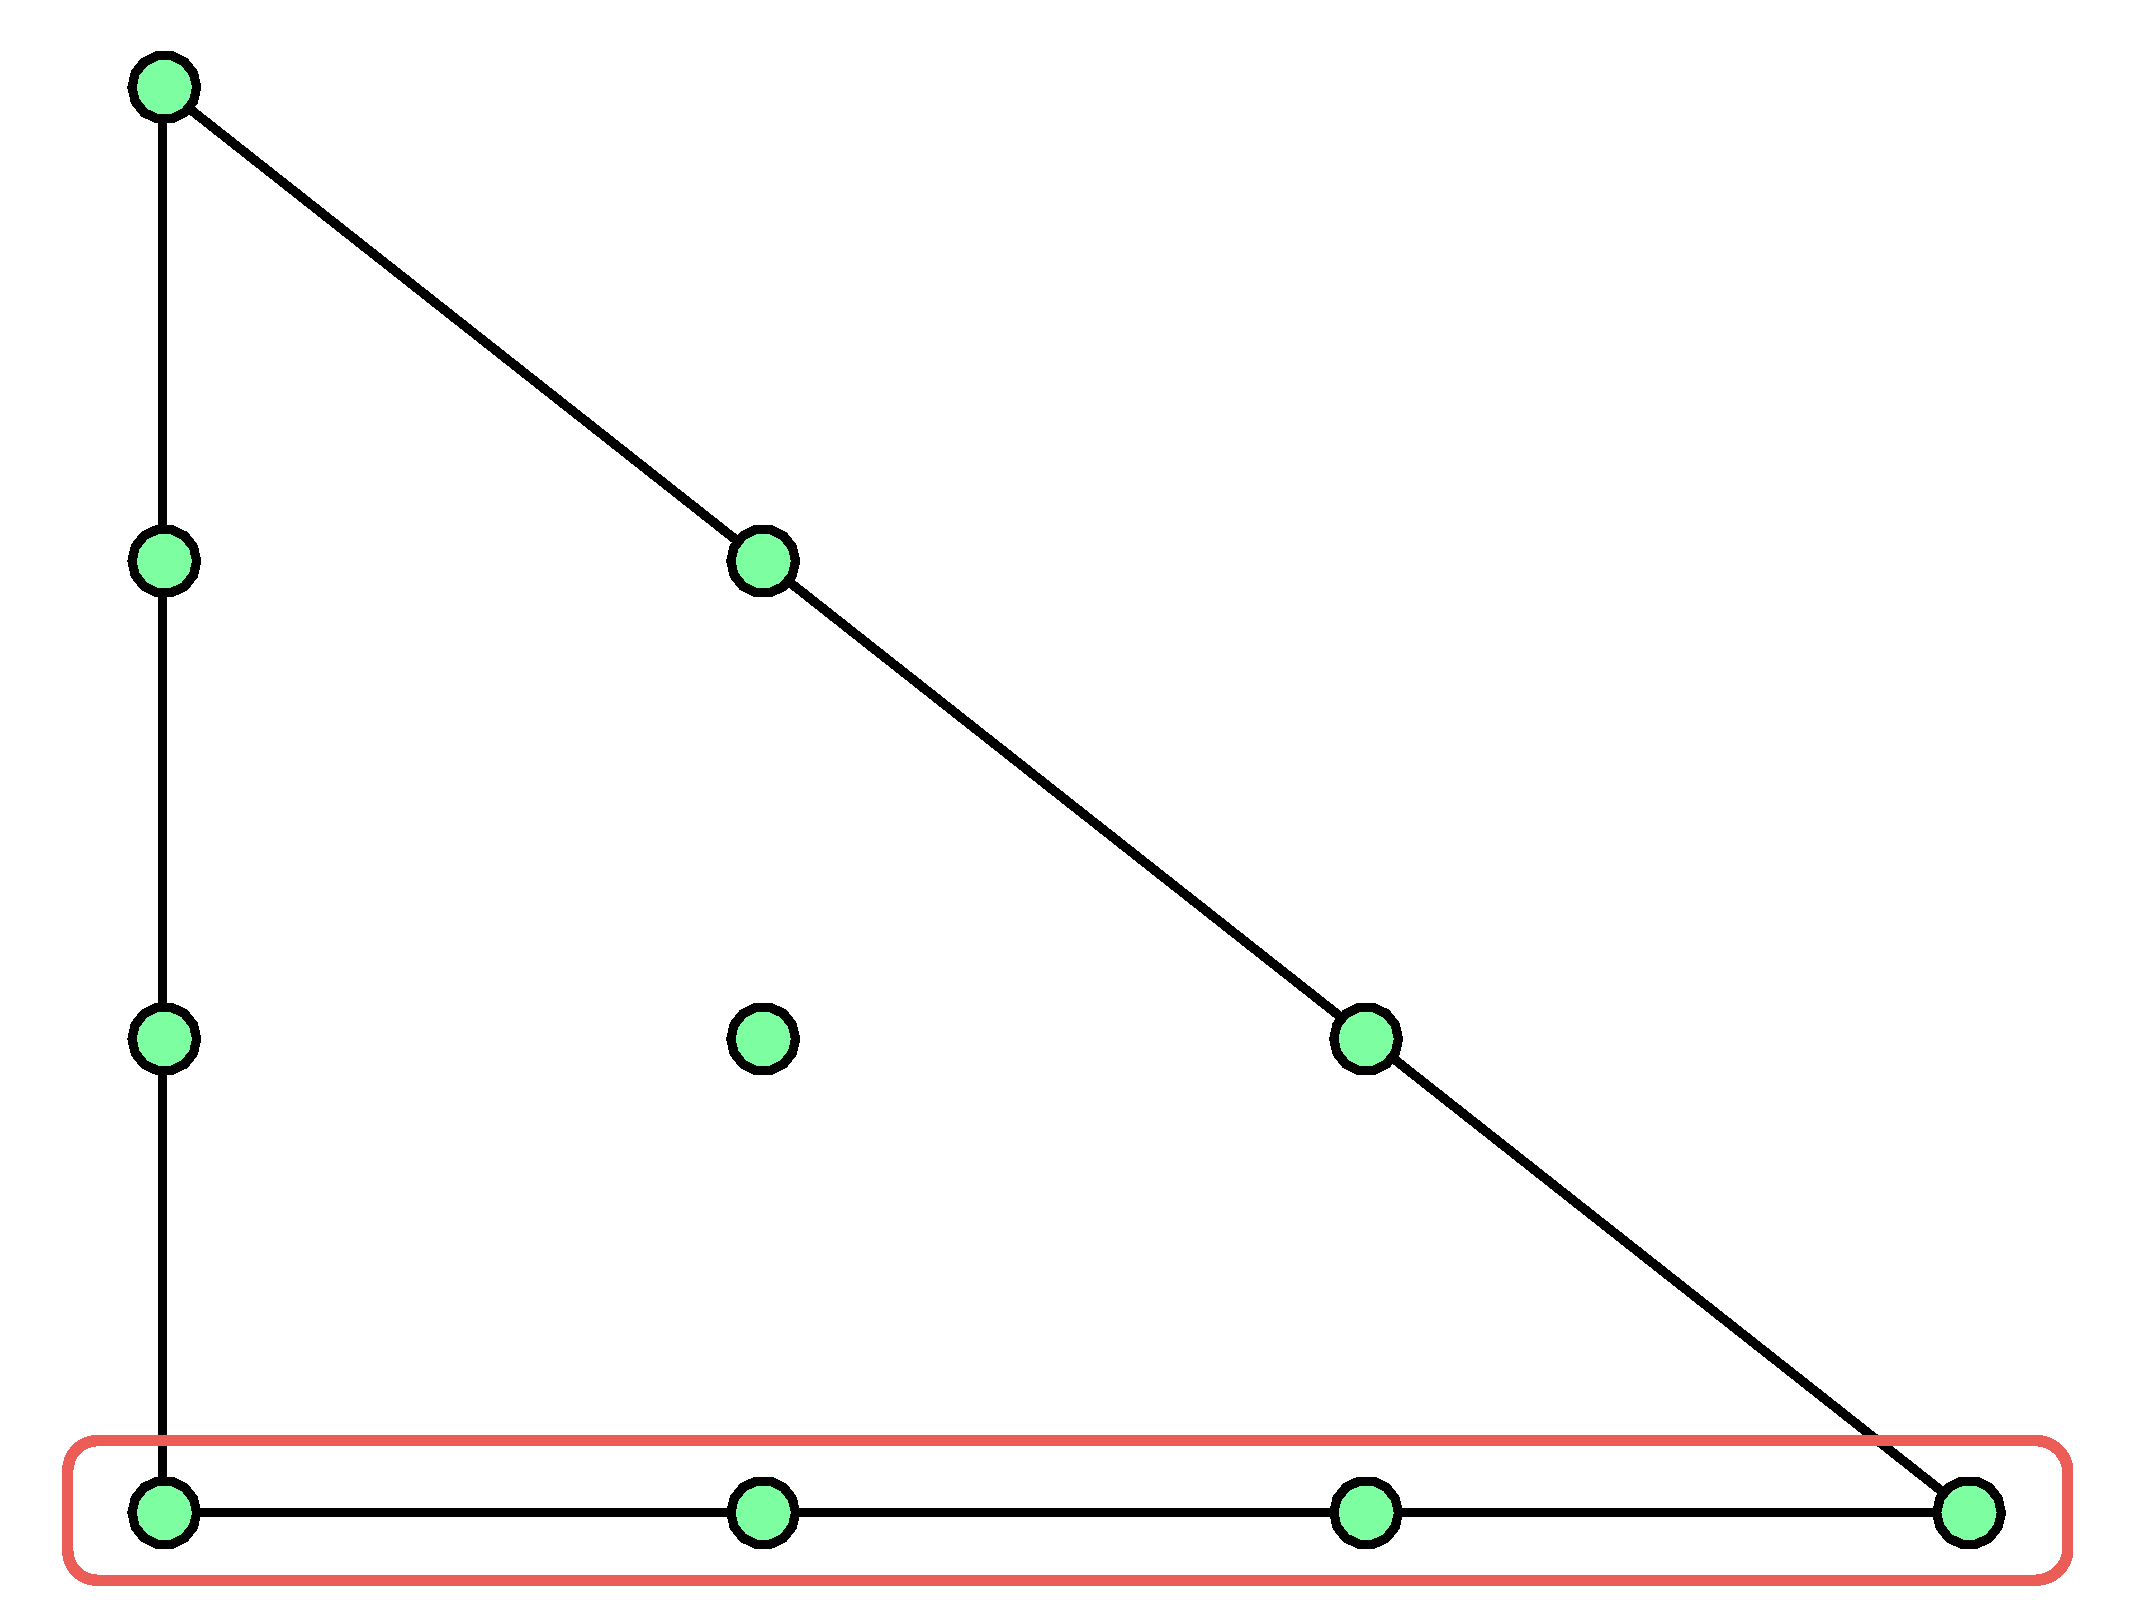
\includegraphics[width=.35\textwidth]{figs/bern_lift_1.pdf}}
\subfloat{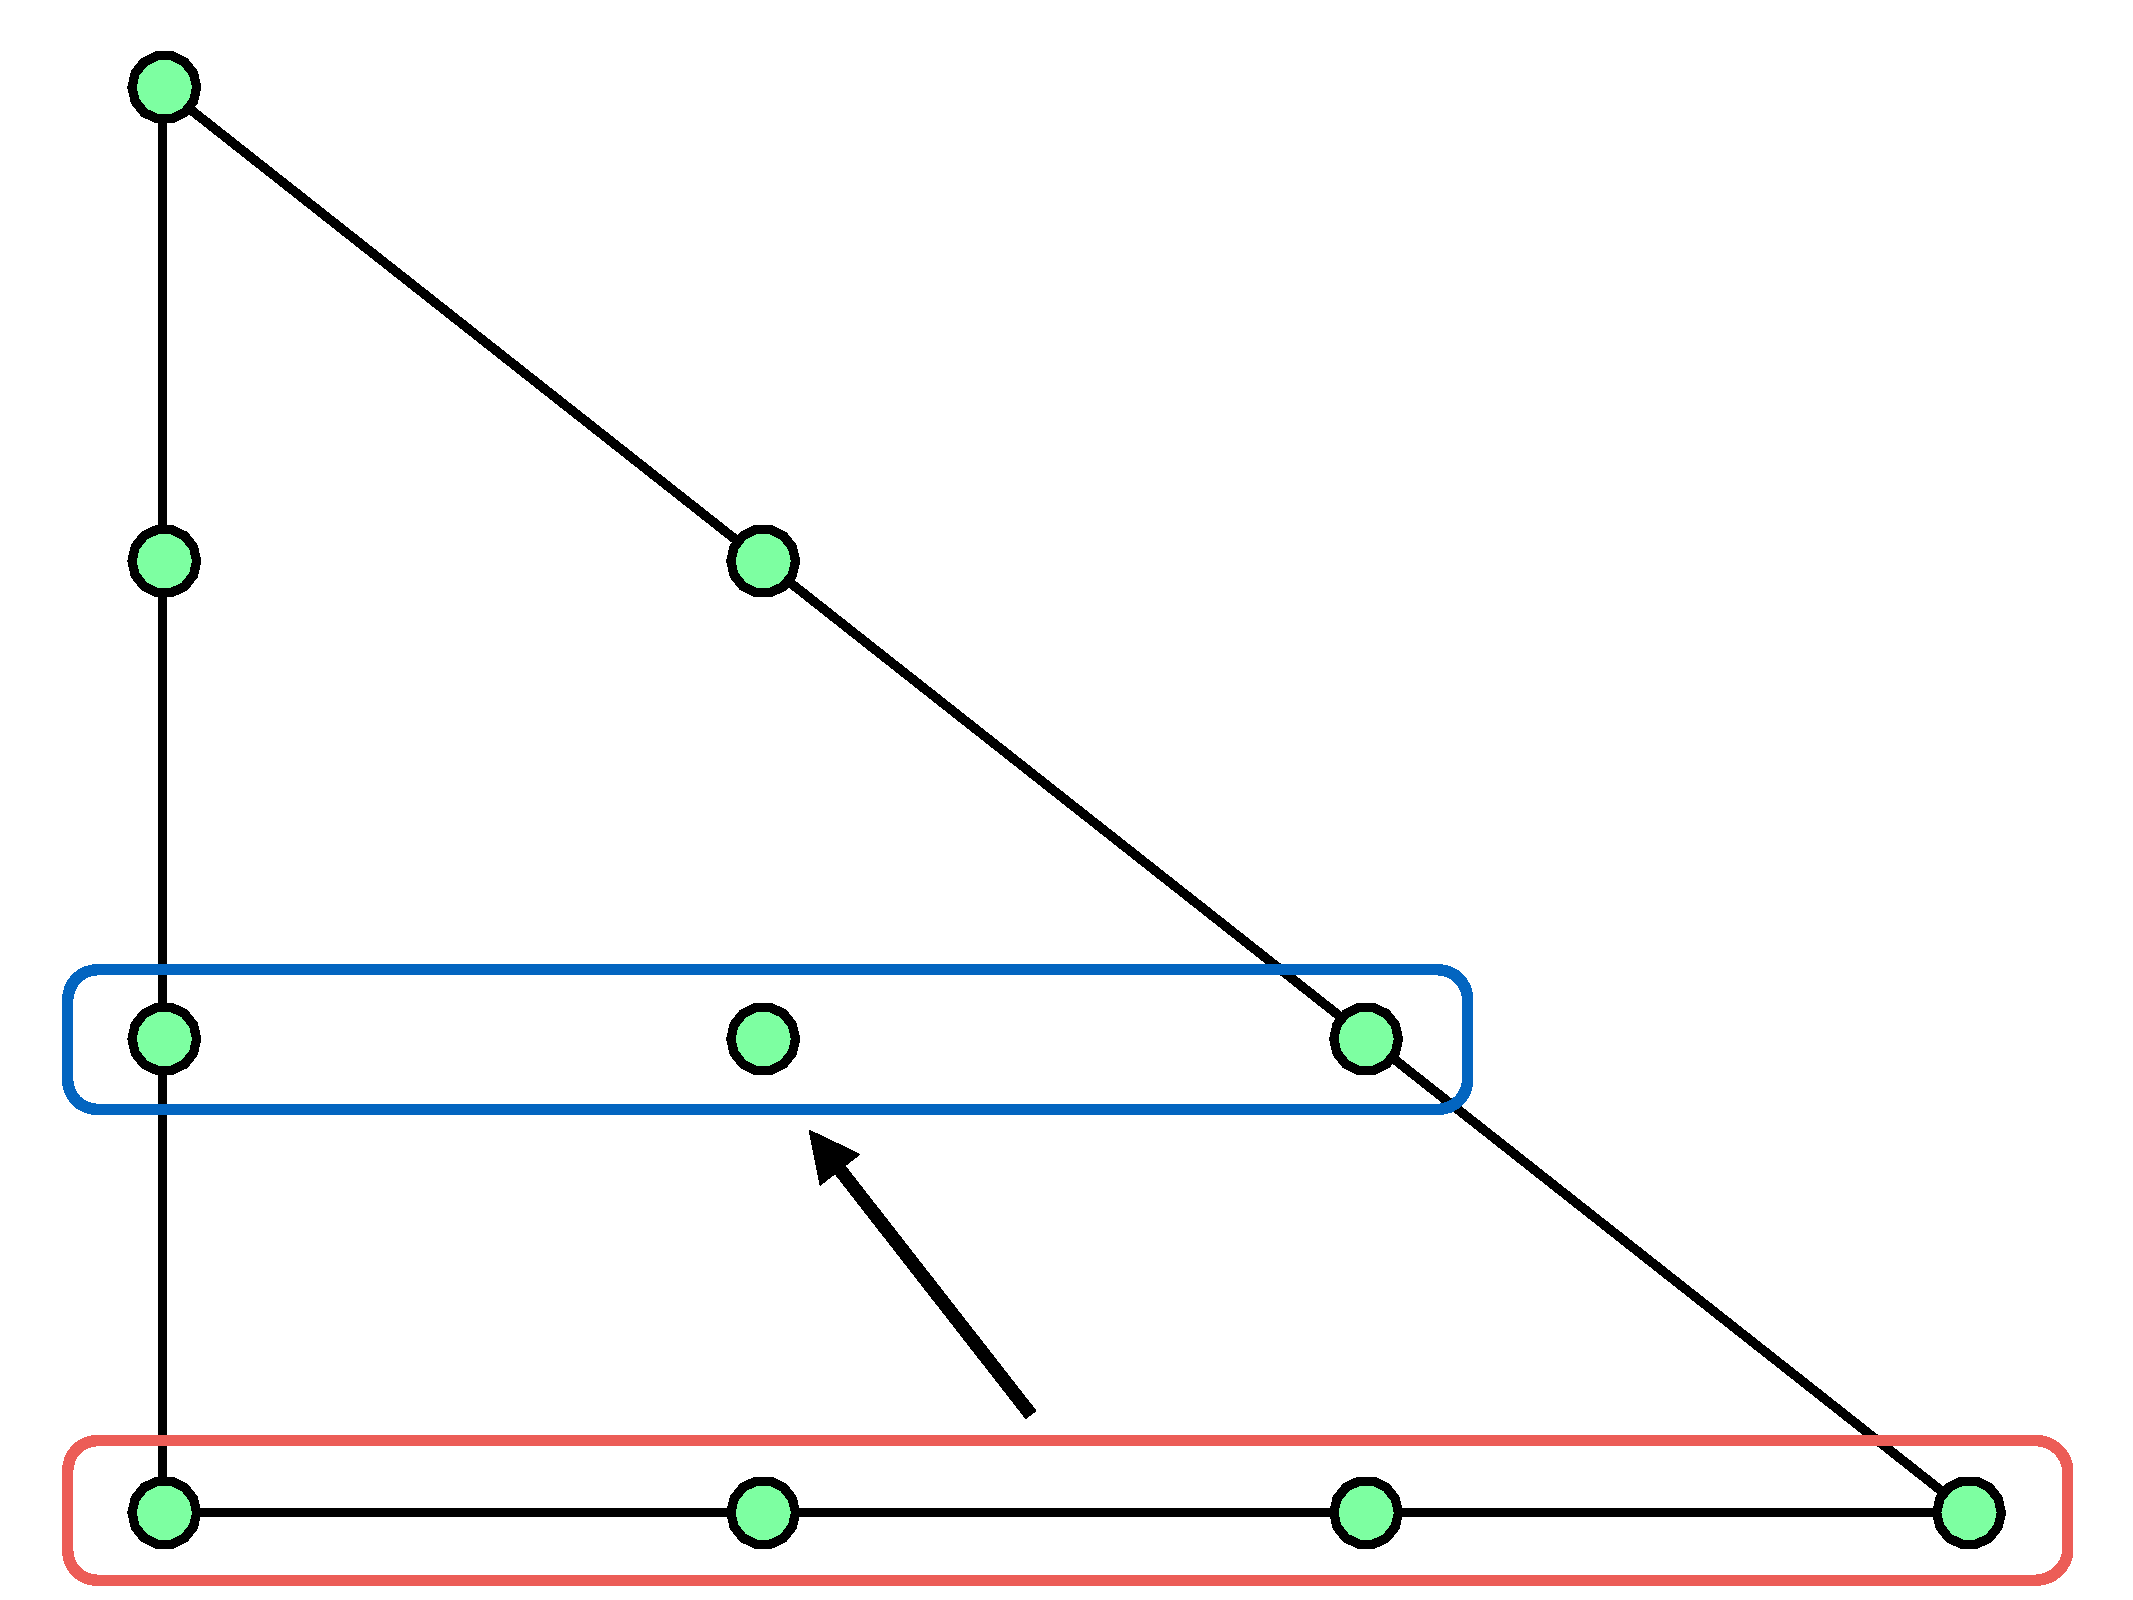
\includegraphics[width=.35\textwidth]{figs/bern_lift_2.pdf}}
\subfloat{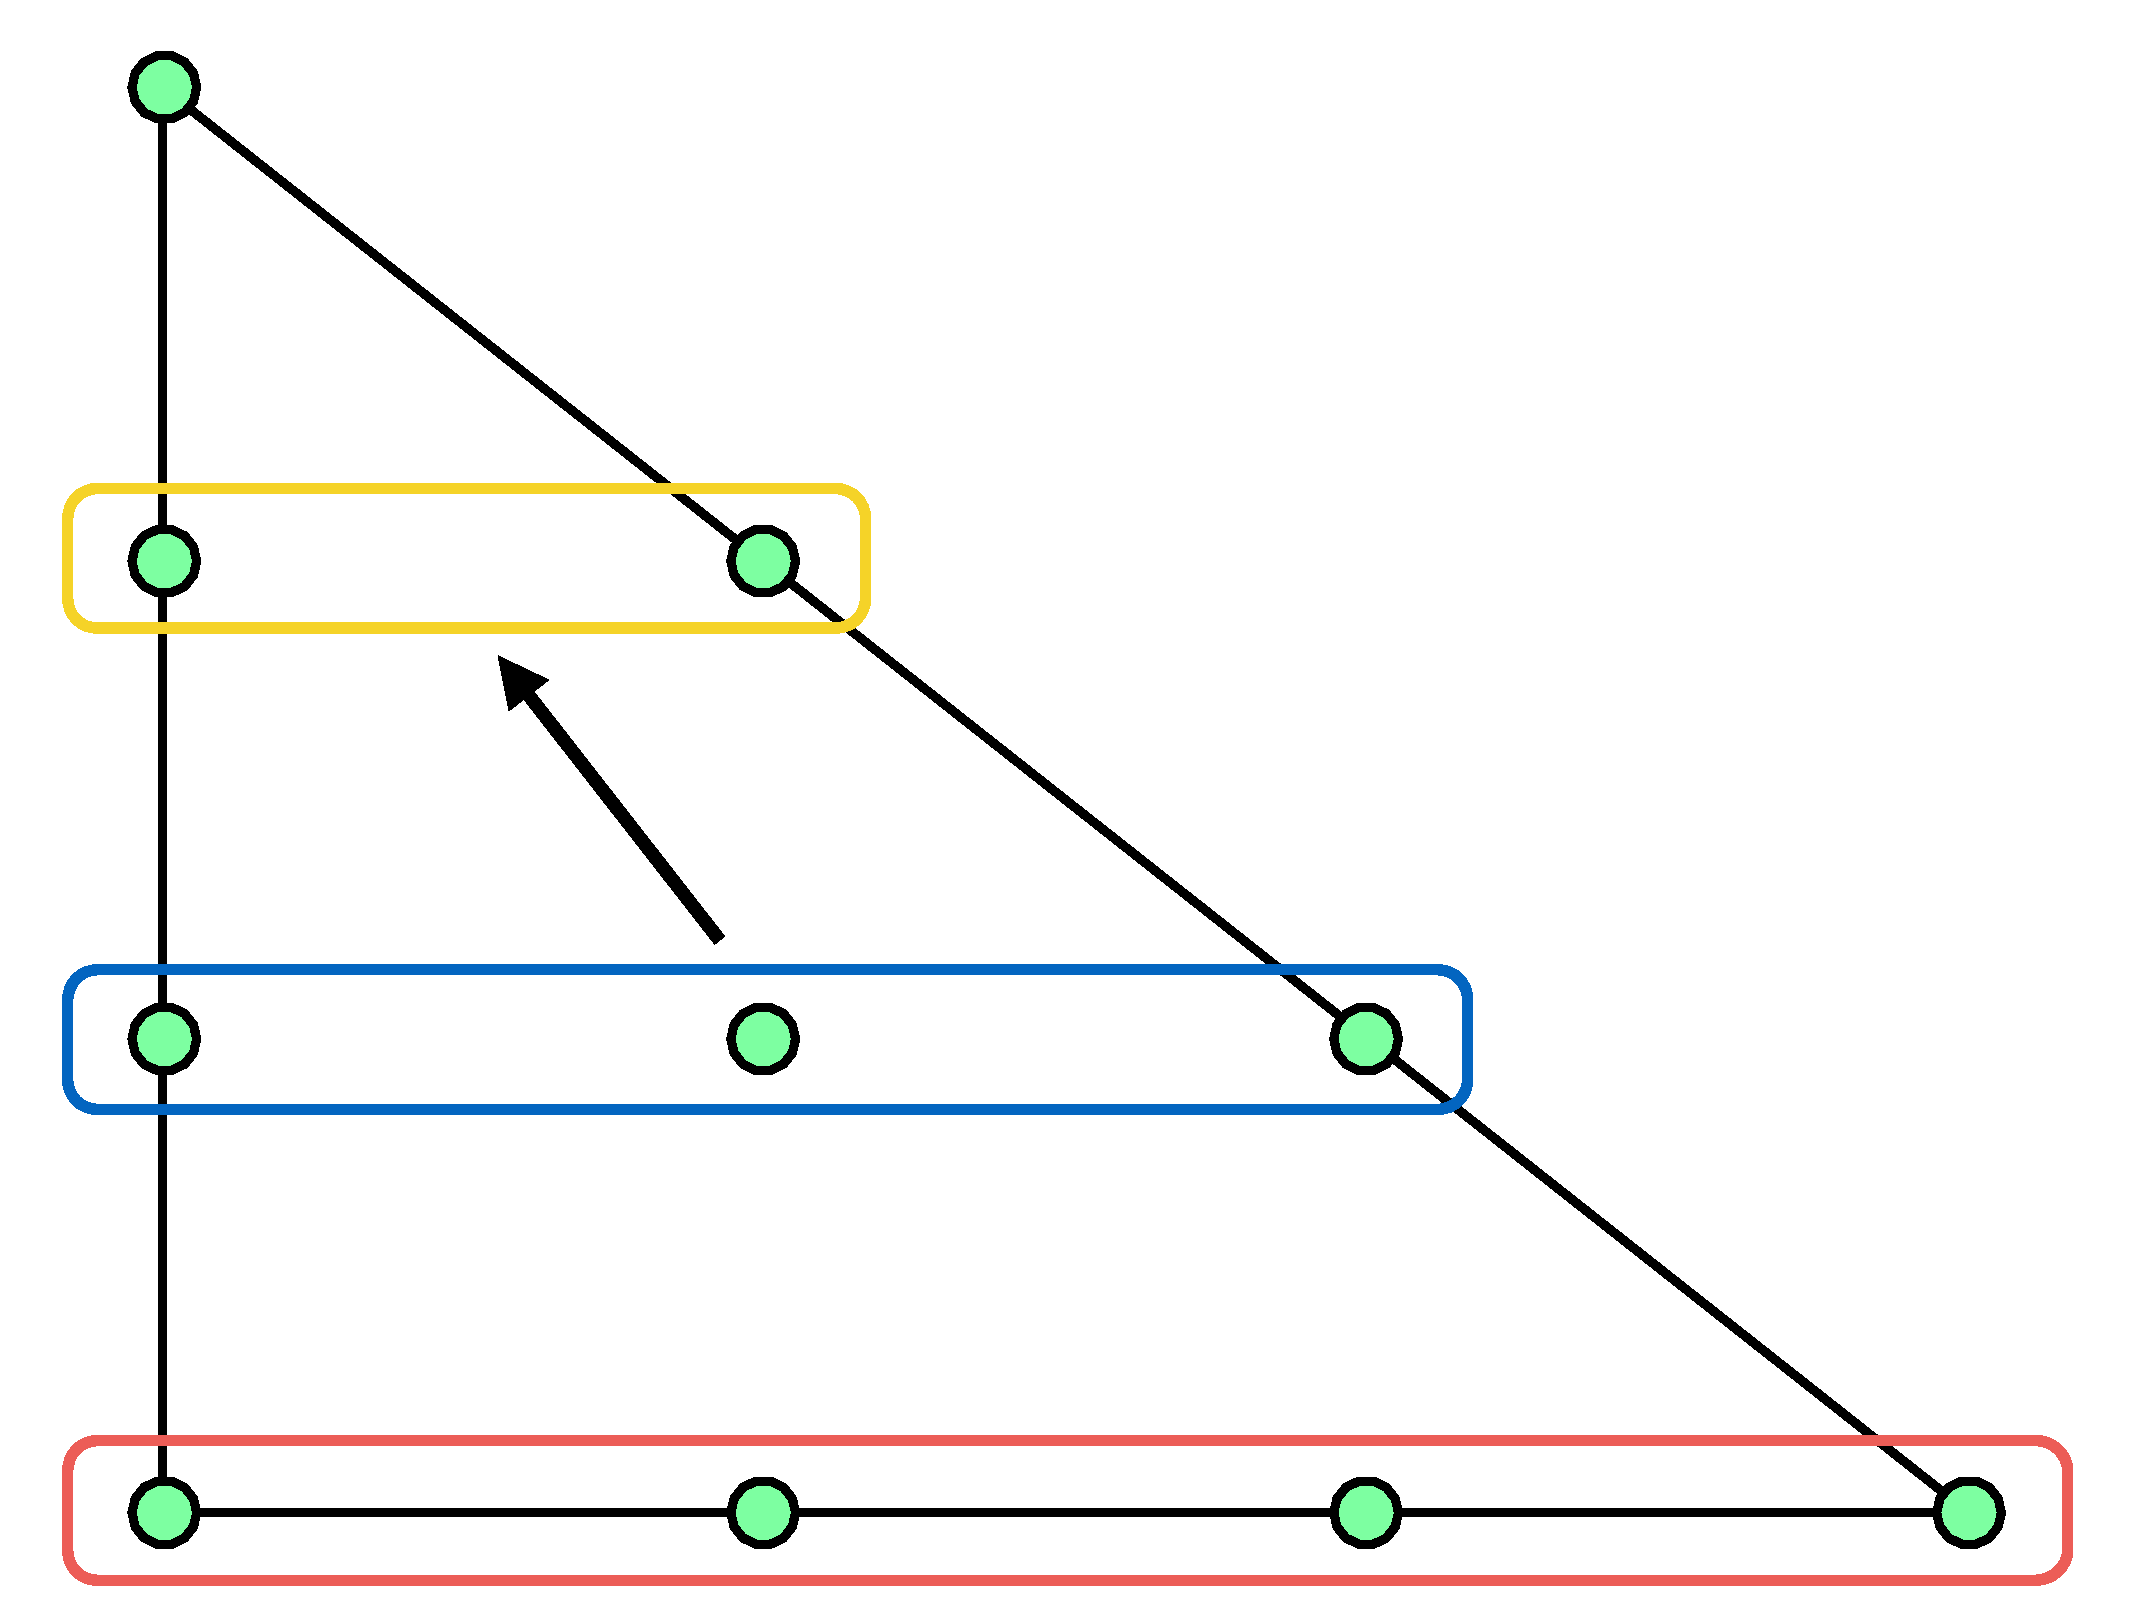
\includegraphics[width=.35\textwidth]{figs/bern_lift_3.pdf}}
\caption*{Optimal $O(N^3)$ complexity ``slice-by-slice'' application of Bernstein lift.}
}
\end{overlayarea}
\end{figure}
\let\thefootnote\relax\footnotetext{\tiny Chan, Warburton 2015.  {GPU-accelerated Bernstein-Bezier discontinuous Galerkin methods for wave propagation} (SISC).}
}

\frame{
\frametitle{BBDG: efficient volume, surface kernels}

\vspace{-.5em}
%\begin{center}
%Bernstein-Bezier DG achieves $\approx 2\times$ speedup at moderate orders,\\ and up to $\approx 6\times$ speedup at high orders.
%\end{center}
%\begin{center}
%Bernstein-Bezier DG achieves $\approx 2\times$ speedup at moderate orders,\\ and up to $4\times$ speedup at high orders.
%\end{center}
\vspace{-1em}
\begin{figure}
\centering
\only<1>{
\hspace{-1em}
\subfloat{
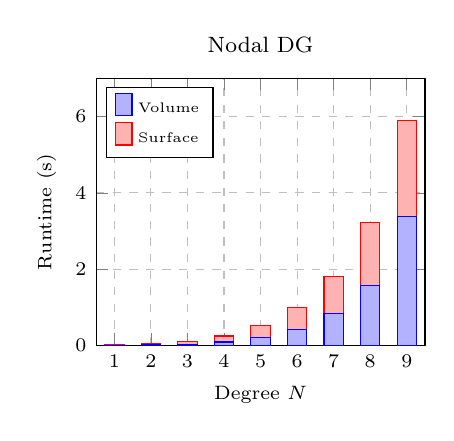
\begin{tikzpicture}
\begin{axis}[
	width=.475\textwidth,
	legend cell align=left,
	title={Nodal DG},
	xlabel={Degree $N$},
	ylabel={Runtime (s)},
	xmin=.5, xmax=9.5,
	ymin=0,ymax=7,
	ybar stacked,
	    bar width=7pt,
	legend style={font=\tiny},	
	xtick={1,2,3,4,5,6,7,8,9},
	legend pos=north west,
	xmajorgrids=true,
	ymajorgrids=true,
	grid style=dashed,
] 
%nodal runtimes
\addplot coordinates{(1,0.00529)(2,0.0135)(3,0.0302)(4,0.0854)(5,0.206)(6,0.41)(7,0.829)(8,1.58)(9,3.39)};
\addplot coordinates{(1,0.0121)(2,0.0403)(3,0.0722)(4,0.158)(5,0.322)(6,0.587)(7,0.987)(8,1.64)(9,2.51)};
%\addplot coordinates{(1,0.009394)(2,0.025607)(3,0.046205)(4,0.080841)(5,0.142045)(6,0.19389)(7,0.27628)(8,0.381)(9,0.5088)};

\legend{Volume, Surface}%, Update}

\end{axis}
\end{tikzpicture}
}
\hspace{1em}
\subfloat{
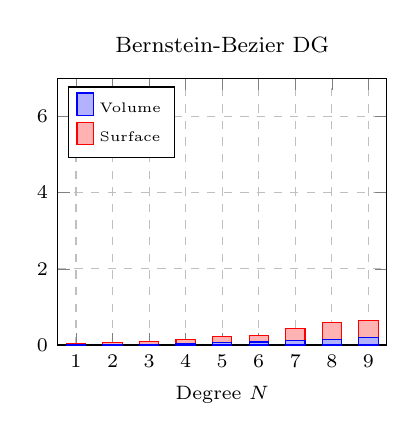
\begin{tikzpicture}
\begin{axis}[
	width=.475\textwidth,
	legend cell align=left,
	title={Bernstein-Bezier DG },
	xlabel={Degree $N$},
	legend style={font=\tiny},	
%	ylabel={Runtime (s)},
	xmin=.5, xmax=9.5,
	ymin=0,ymax=7,
	ybar stacked,
	    bar width=7pt,
	xtick={1,2,3,4,5,6,7,8,9},
	legend pos=north west,
	xmajorgrids=true,
	ymajorgrids=true,
	grid style=dashed,
] 
%bern runtimes
\addplot 
coordinates{(1,0.00564)(2,0.0119)(3,0.0203)(4,0.034)(5,0.0593)(6,0.0791)(7,0.112)(8,0.155)(9,0.204)};
\addplot 
coordinates{(1,3.45E-02)(2,5.15E-02)(3,6.61E-02)(4,1.03E-01)(5,1.76E-01)(6,1.73E-01)(7,3.32E-01)(8,4.48E-01)(9,4.31E-01)};
%\addplot 
%coordinates{(1,0.0093767)(2,0.0255921)(3,0.04623)(4,0.081)(5,0.14229)(6,0.194133)(7,0.277041)(8,0.38163)(9,0.50694)};

\legend{Volume, Surface}%, Update}

\end{axis}
\end{tikzpicture}
}
%\caption*{Per-kernel runtimes for nodal and Bernstein-Bezier bases.  Runtimes are recorded for ten RK4 timesteps on a mesh of 98304 elements.}
%\caption*{Kernel runtimes for Naive nodal, Blocked nodal, and Bernstein-Bezier DG implementations (50 RHS evaluations, 98304 elements).}
%\caption*{Kernel runtimes for Standard nodal, Blocked nodal, and Bernstein-Bezier DG implementations (50 RHS evaluations, 98304 elements).}
%\caption*{DG runtimes for 50 timesteps, 98304 elements.}
}

% maybe comment out? speedup
\only<2>{
\subfloat{
\begin{tikzpicture}
\begin{axis}[
	width=.5\textwidth,
	legend cell align=left,
	title={BBDG speedup over nodal DG},
	xlabel={Degree $N$},
	ylabel={Speedup},
	xmin=.5, xmax=9.5,
	ymin=0,ymax=8,%17.5,	
        ybar=2*\pgflinewidth,
    bar width=3pt,
	xtick={1,2,3,4,5,6,7,8,9},
	ymin=0,
	legend pos=north west,
	legend style={font=\tiny},
	ymajorgrids=true,
	grid style=dashed,
] 
%speedup V/S
%\addplot table[x=N, y=V] from \runtimeOptNaive;
%\addplot table[x=N, y=S] from \runtimeOptNaive;
\addplot table[x=N, y=V] from \runtimeSpeedupBest;
\addplot table[x=N, y=S] from \runtimeSpeedupBest;
%\addplot table[x=N, y=T] from \runtimeOptNaive;
%\addplot table[x=N, y=Vopt] from \datatable;
\addplot+[draw=black,line legend, very thick,smooth,dashed] coordinates{(0,1)(10,1)};

%\legend{Volume, Surface, Total, Reference (no speedup)}
\legend{Volume, Surface}%, Total}%, No speedup}
\end{axis}
\end{tikzpicture}

}

%\caption*{Ratio of runtimes of volume/surface kernels and total RHS evaluation using a Bernstein-Bezier basis instead of nodal polynomials.}
%\caption*{Speedups achieved over nodal DG by using a Bernstein-Bezier basis.}
}
%\caption*{Bernstein-Bezier DG achieves $\approx 2\times$ speedup at moderate orders,\\ and up to $4\times$ speedup at high orders.}
\end{figure}
%\only<1>{\vspace{-.25em}}
%\only<2>{\vspace{-.5em}}
\vspace{-.75em}
\[
\underbrace{\td{\mathbf{u}}{t}}_{\text{Update kernel}} = \underbrace{\mathbf{D}_x \mathbf{u}}_{\text{Volume kernel}} + \underbrace{\sum_{\text{ faces}}\mathbf{L}_f \LRp{\rm flux}}_{\text{Surface kernel}}, \quad \mathbf{L}_f = \mathbf{{M}}^{-1}\mathbf{{M}}_f.
\]
}

\frame{
\frametitle{BBWADG: polynomial multiplication and projection}
\setcounter{subfigure}{0}
\vspace{-1em}
\begin{figure}
\centering
\hspace{-1em}
\subfloat[Exact $c^2$]{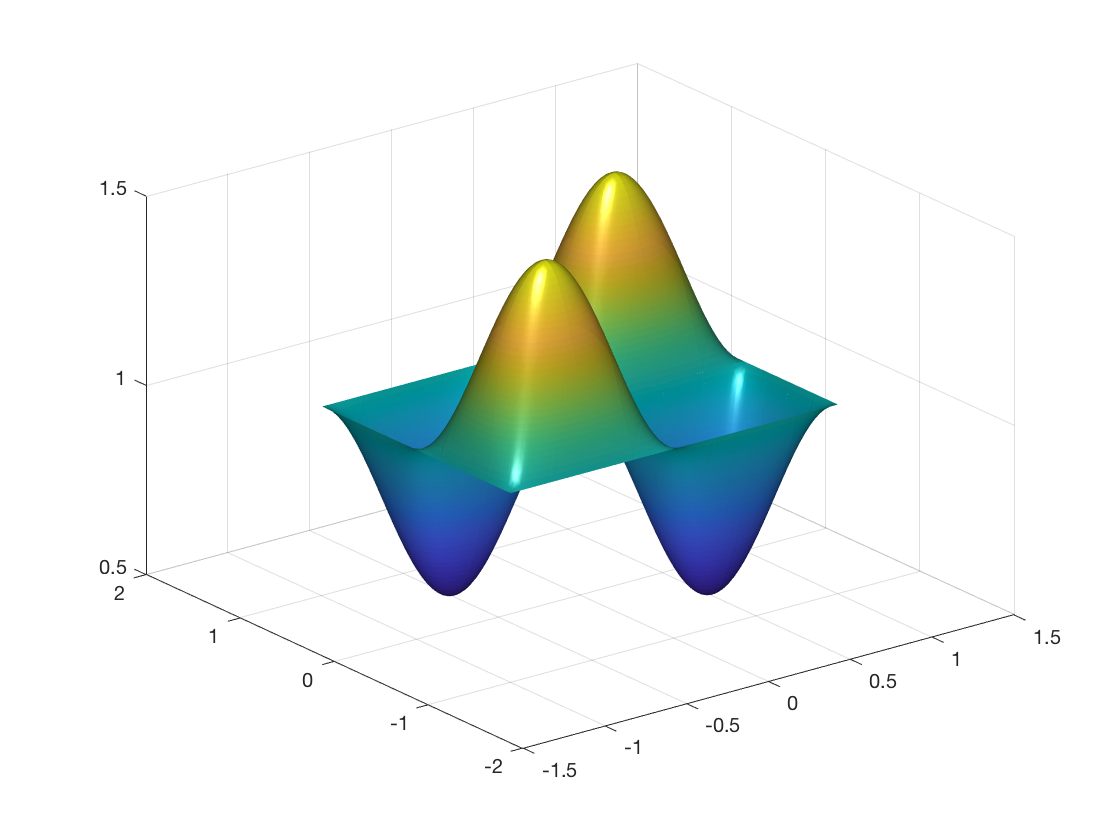
\includegraphics[width=.35\textwidth]{figs/cfunEx.png}}
\hspace{-1em}
\subfloat[$M=0$ approximation]{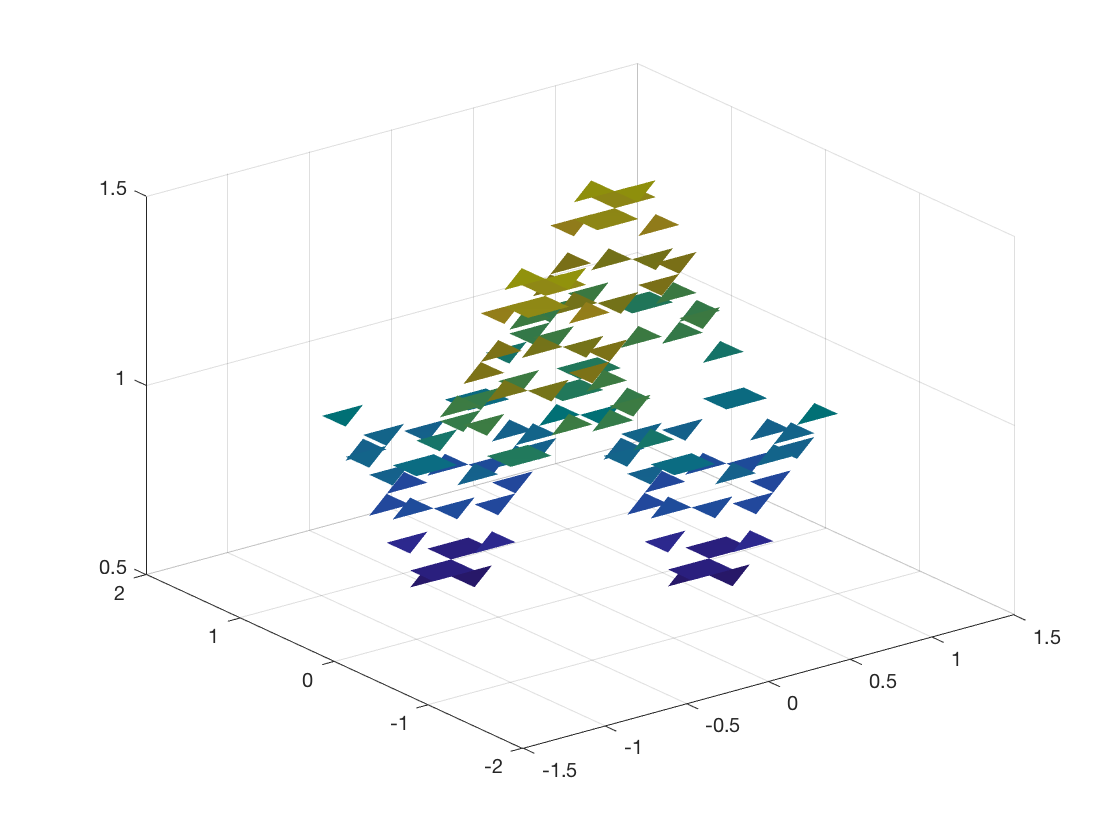
\includegraphics[width=.35\textwidth]{figs/cfun_M0.png}}
\hspace{-1em}
\subfloat[$M=1$ approximation]{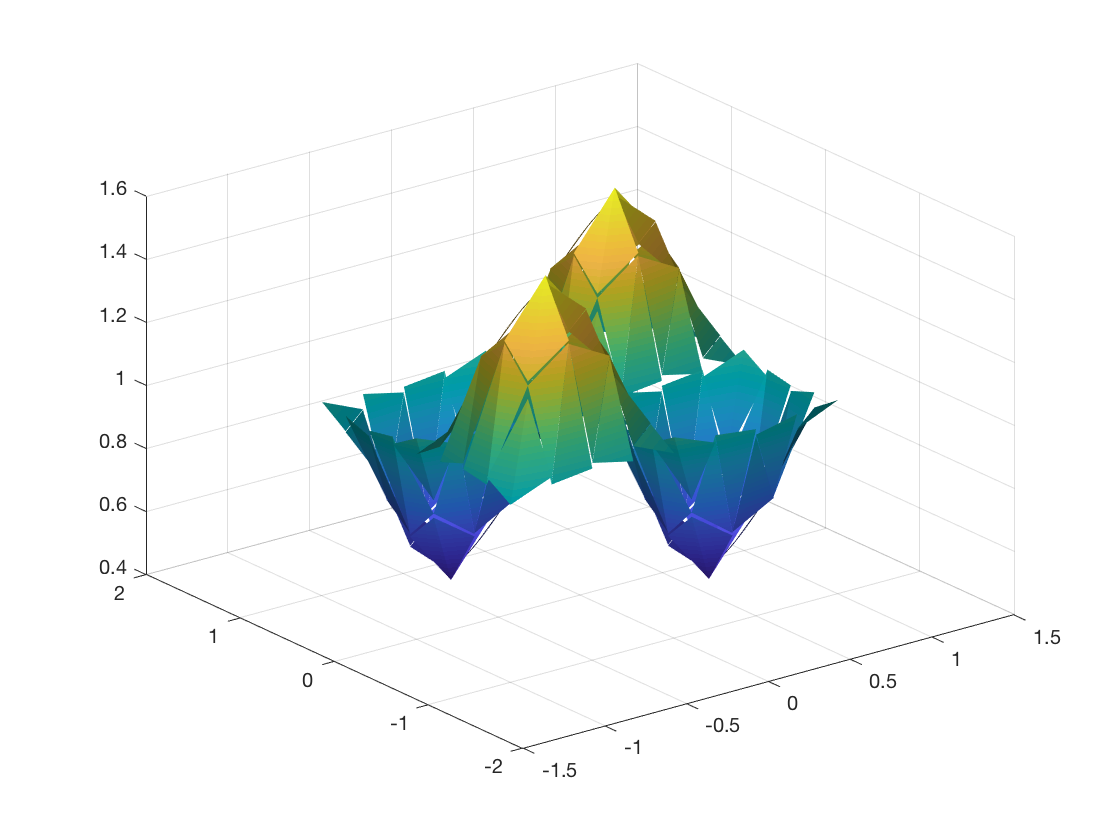
\includegraphics[width=.35\textwidth]{figs/cfun_M1.png}}
\end{figure}

\begin{itemize}
\item WADG: can reuse fast Bernstein volume and surface kernels.
\vspace{.5em}
\item $O(N^6)$ update kernel: $\bm{V}_q$ interpolates $u(\bm{x})$ to quadrature points, scale by $c^2(\bm{x})$ at quadrature points, apply $\bm{P}_q$ to project back to $P^N$.
\vspace{.5em}
\item New approach: approx.\ $c^2(\bm{x})$ with degree $M$ polynomial, use fast Bernstein algorithms for polynomial multiplication and projection.
\end{itemize}
}

%\frame{
%\frametitle{Quadrature-based WADG}
%
%}

\frame{
\frametitle{Fast Bernstein polynomial multiplication}
\begin{figure}
\centering
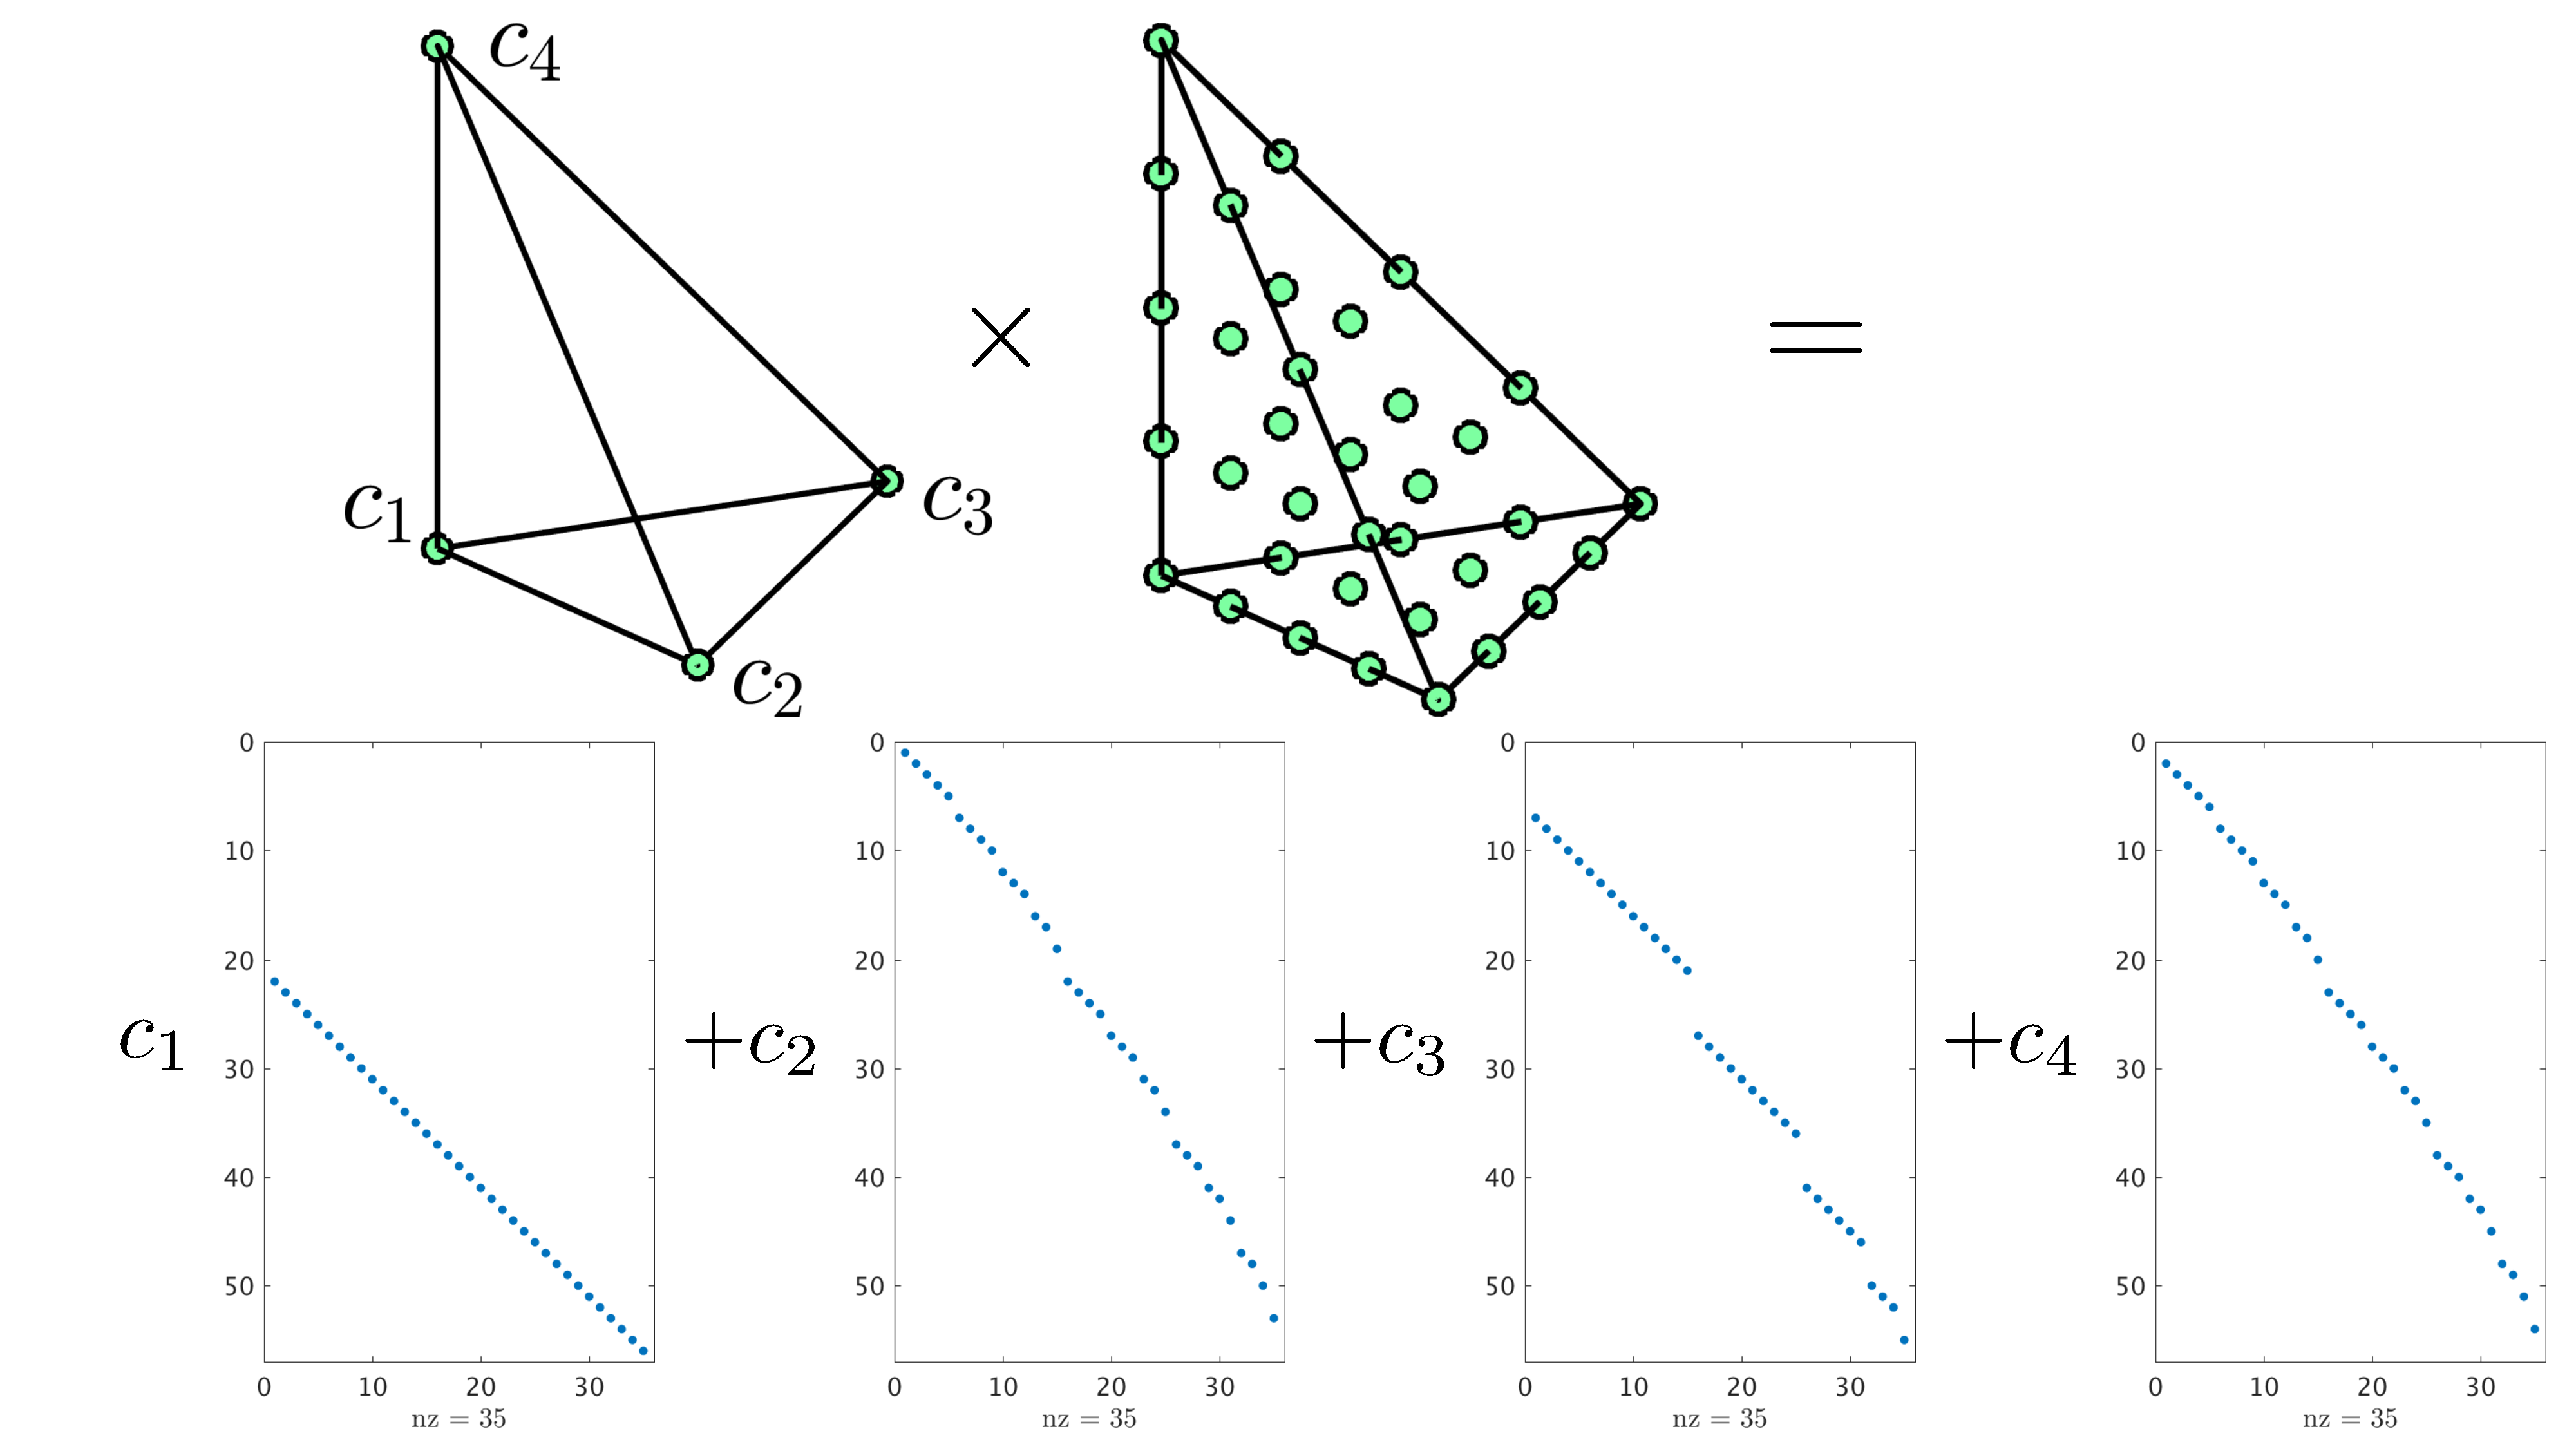
\includegraphics[width=.95\textwidth]{figs/polymult.pdf}
\caption*{Bernstein polynomial multiplication: for fixed $M$, $O(N^3)$ complexity.}
\end{figure}

}

\frame{
\frametitle{Fast Bernstein polynomial projection}

\begin{itemize}
%\item Polynomial multiplication: $c^2(\bm{x})u(\bm{x}) \in P^{M+N}$.
%\[
%\sum_{j=1}^{M_p} c_j \bm{C}_j \bm{u}.
%\]
\item Given $c^2(\bm{x})u(\bm{x})$ as a degree $(N+M)$ polynomial, apply $L^2$ projection matrix $\bm{P}^{N+M}_N$ to reduce to degree $N$.  
\vspace{.5em}
\item Polynomial $L^2$ projection matrix $\bm{P}^{N+M}_N$ under Bernstein basis: 
\[
\bm{P}^{N+M}_N = %\sum_{j=0}^N c_j\bm{E}_{N-j}^N\LRp{\bm{E}_{N-j}^{N+M}}^T = 
\underbrace{\sum_{j=0}^N c_j\bm{E}_{N-j}^N \LRp{\bm{E}_{N-j}^{N}}^T}_{\tilde{\bm{P}}_N}\LRp{\bm{E}_{N}^{N+M}}^T
\]
\item ``Telescoping'' form of $\tilde{\bm{P}}_N$: \textcolor{red}{$O(N^4)$ complexity}, more GPU-friendly.
\[
\left(c_0\bm{I}+\bm{E}^N_{N-1}\left(c_1\bm{I}+\bm{E}^{N-1}_{N-2}\left(c_2\bm{I}+\cdots\right)\left(\bm{E}^{N-1}_{N-2}\right)^T\right)\left(\bm{E}^N_{N-1}\right)^T\right)
\]
%\item Apply $N$ (sparse) degree elevation matrices $\bm{E}^{j}_{j-1}$: $O(N^4)$ complexity.
\end{itemize}
}

\frame{
\frametitle{Sketch of GPU algorithm for $\tilde{P}_N$}% for $N=3$}
\vspace{-.75em}
\begin{figure}
\centering
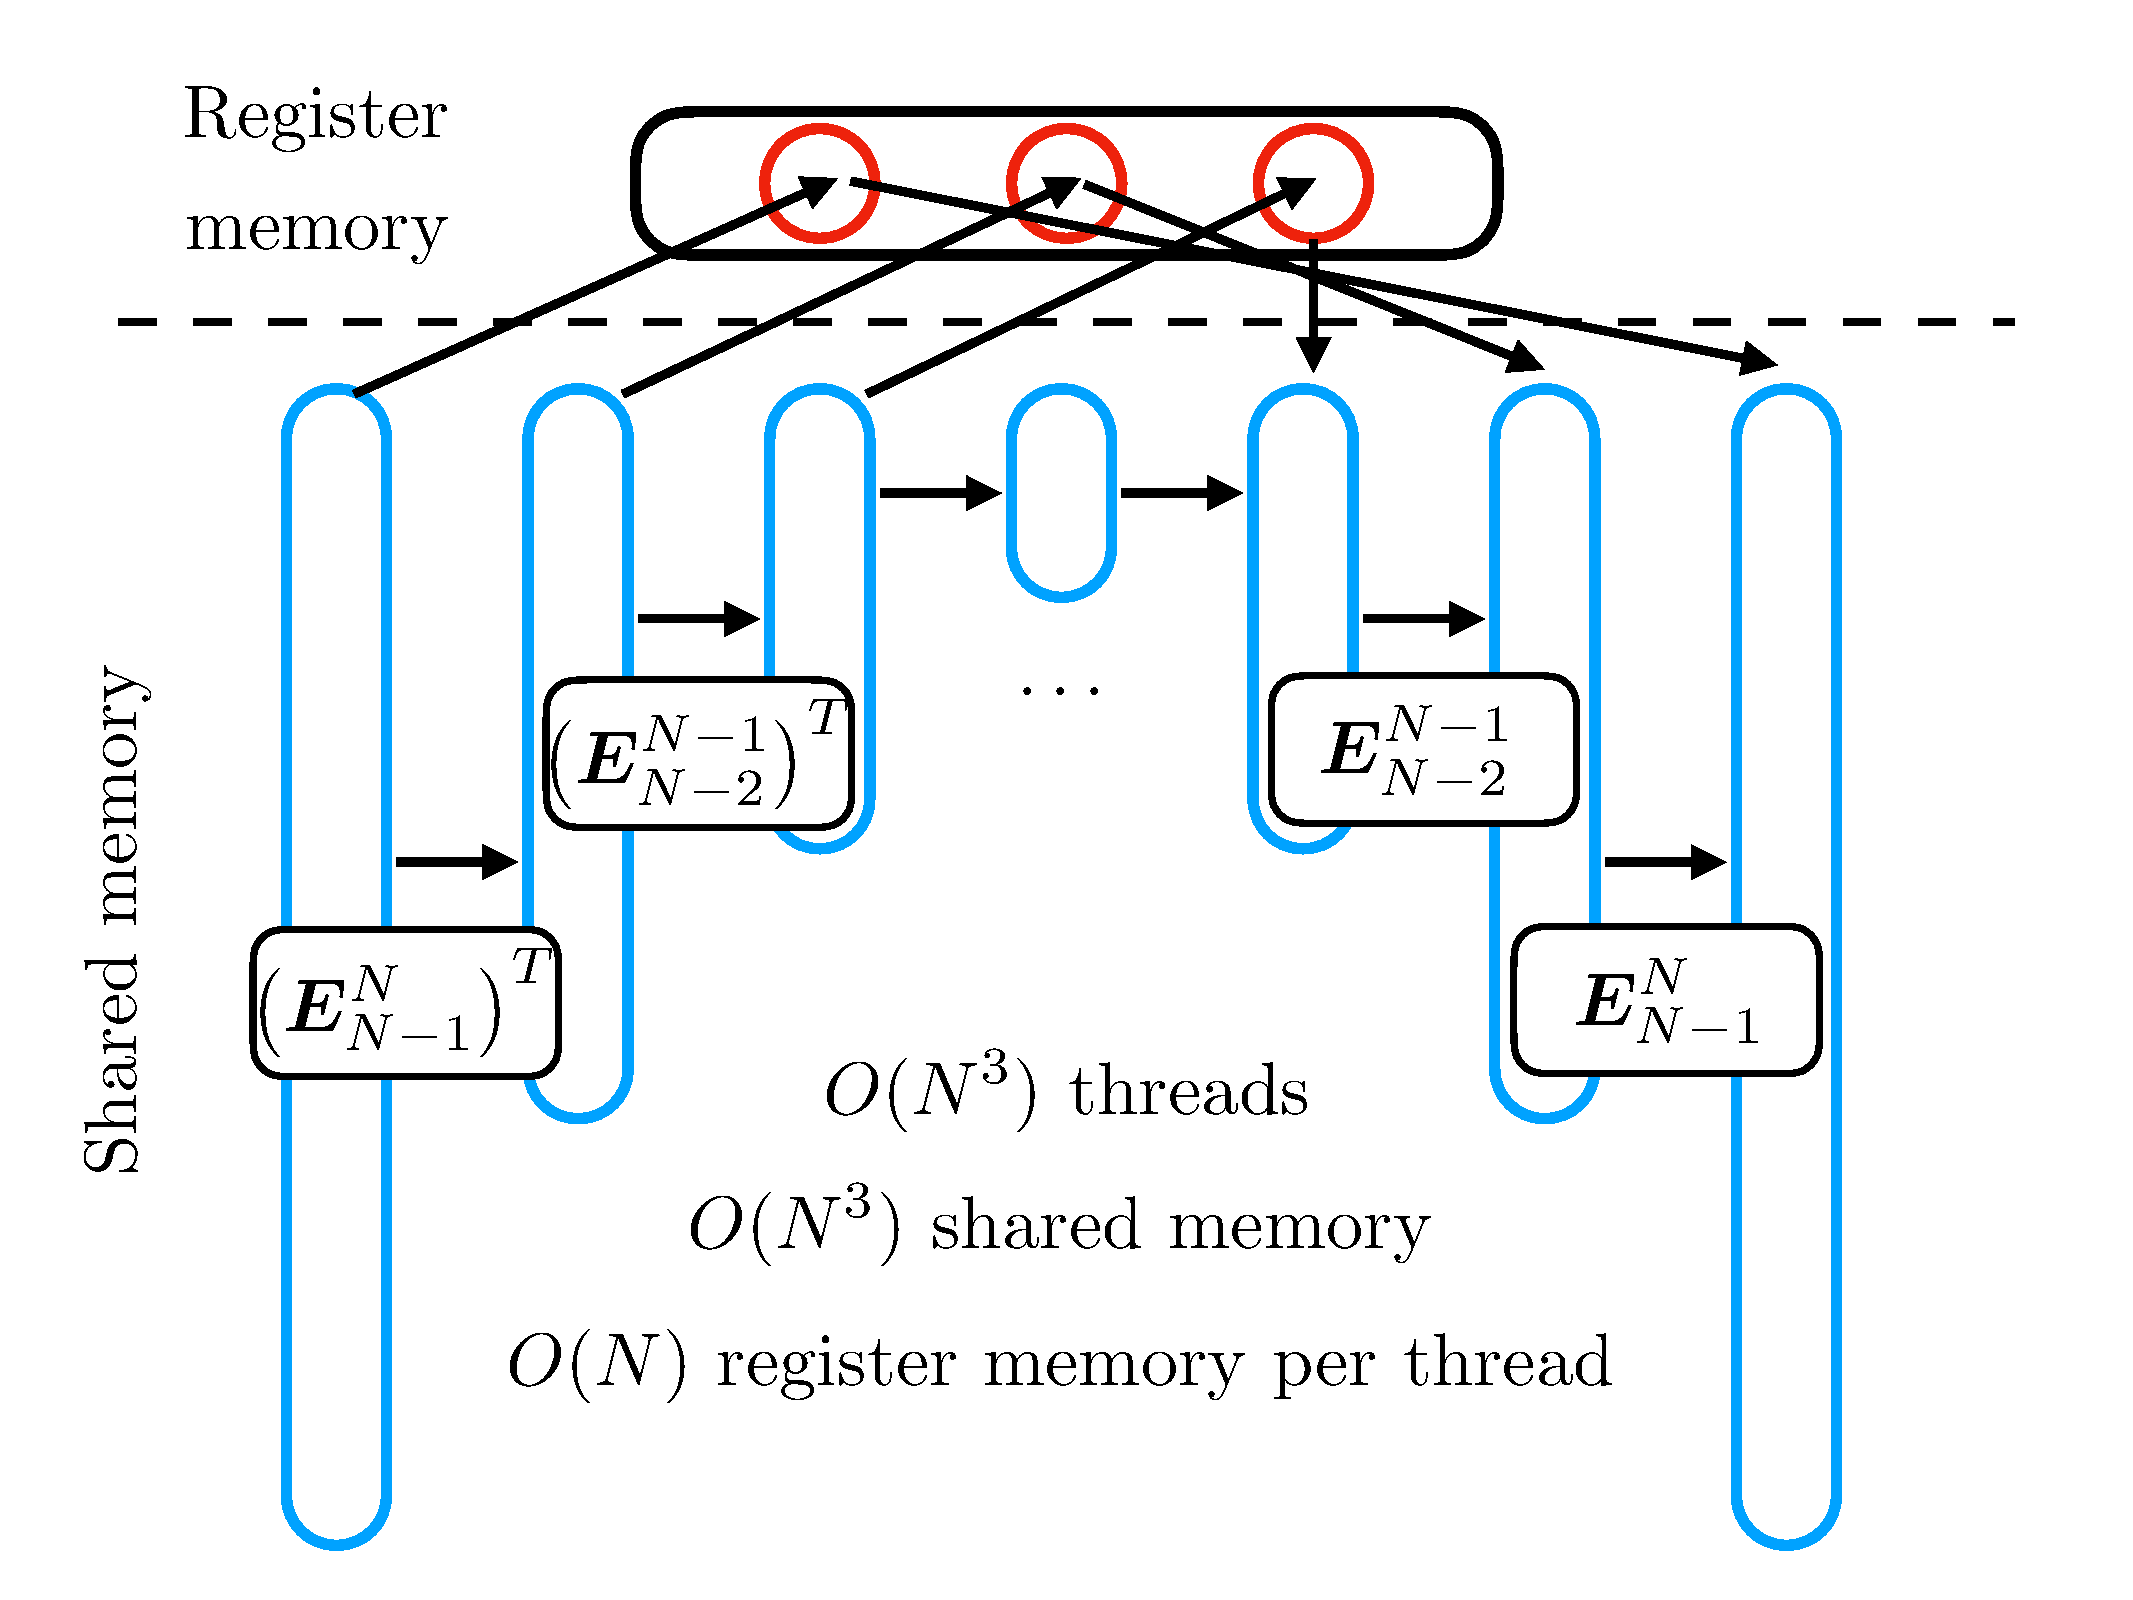
\includegraphics[width=.75\textwidth]{figs/bbproj.pdf}
\end{figure}
\vspace{-.5em}
\[
\left(c_0\bm{I}+\bm{E}^N_{N-1}\left(c_1\bm{I}+\bm{E}^{N-1}_{N-2}\left(c_2\bm{I}+\cdots\right)\left(\bm{E}^{N-1}_{N-2}\right)^T\right)\left(\bm{E}^N_{N-1}\right)^T\right)
\]
}

\frame{
\frametitle{BBWADG: approximating $c^2$ and accuracy}

\begin{figure}
\centering
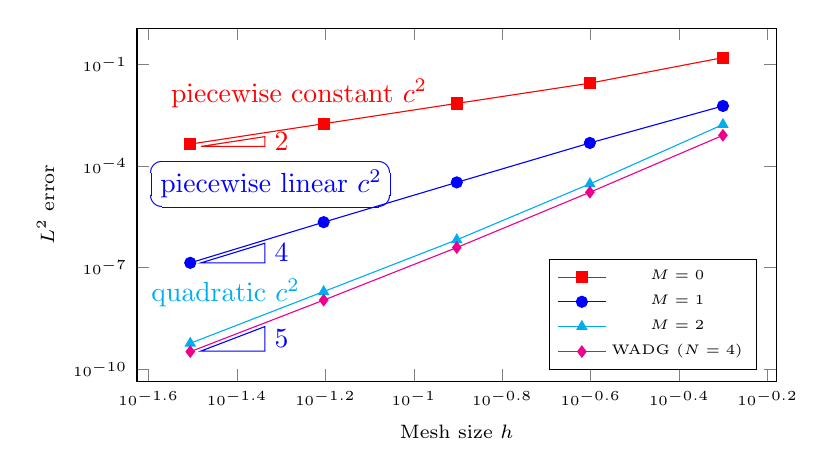
\begin{tikzpicture}
\begin{loglogaxis}[
width=0.8\textwidth,
height=0.5\textwidth,
title style = {font=\small},
%title = {Convergence of Bernstein-B\'ezier WADG ($N=4$)},
xlabel= Mesh size $h$,
ylabel= $L^2$ error,
ticklabel style = {font=\tiny},
%xtick = data,
%xticklabels={$2$,$3$,$4$,$5$,$6$,$7$,$8$},
%ymin=0.0000000001,ymax=1,
legend style={font=\tiny},
legend pos = south east
]
\addplot[color=red,mark=square*] coordinates {
	(0.5,0.1575135 )
	(0.25,0.02778378)
	(0.125,0.00701356)
	(0.0625,0.001763432)
	(0.0312,0.0004414745)
	};

%\addplot[color=blue,mark=otimes*] coordinates {
%	(0.5,0.05666667 )
%	(0.25,0.01566016)
%	(0.125,0.0007522236)
%	(0.0625,0.0000660265)
%	(0.0312,0.0000042542)
%	};

\addplot[color=blue,mark=otimes*] coordinates {
	(0.5,0.00590602 )
	(0.25,0.0004771556)
	(0.125,0.000032725844293)
	(0.0625,0.0000021917583)
	(0.0312,0.000000138034585)
	};

%\addplot[color=red,mark=triangle*] coordinates {
%	(0.5,0.03162 )
%	(0.25,0.054654)
%	(0.125,0.01402863)
%	(0.0625,0.00065991)
%	(0.0312,0.000058665)
%	};
\addplot[color=cyan,mark=triangle*] coordinates {
	(0.5,0.001672084 )
	(0.25,0.000029571618)
	(0.125,0.000000659821706)
	(0.0625,0.000000019551547)
	(0.0312,0.000000000582975)
	};
%\addplot[color=blue,mark=diamond*] coordinates {
%	(0.5,0.098363 )
%	(0.25,0.0331846)
%	(0.125,0.0541294)
%	(0.0625,0.01390139)
%	(0.0312,0.000656537)
%	};
\addplot[color=magenta,mark=diamond*] coordinates {
	(0.5,0.00080421 )
	(0.25,0.0000167281)
	(0.125,0.00000039029)
	(0.0625,0.0000000109402)
	(0.0312,0.000000000329775504)
	};

\logLogSlopeTriangle{0.2}{0.1}{0.085}{5}{blue};
\logLogSlopeTriangle{0.2}{0.1}{0.665}{2}{red};
\logLogSlopeTriangle{0.2}{0.1}{0.335}{4}{blue};
%\addplot[dashed, color=black,mark=diamond*] coordinates {
%	(0.5,3.1250000000000)
%	(0.25,0.09765625)
%	(0.125,0.0030517578)
%	(0.0625,0.00009536743)
%	(0.0312,0.000002956466553)
%	};

\node[above,red] at (axis cs: .055,.00275){piecewise constant $c^2$};
\node[above,blue] at (axis cs: .0475,.000003){\ovalbox{piecewise linear $c^2$}};
\node[above,cyan] at (axis cs: .0375,.0000000035){quadratic $c^2$};
\legend{$M=0$,$M=1$, $M=2$, WADG ($N=4$)}
\end{loglogaxis}
\end{tikzpicture}
%\caption*{Convergence of BBWADG for $M=0, 1,2$ and $N=4$.}
\end{figure}
\begin{center}
Approximating smooth $c^2(\bm{x})$ using $L^2$ projection:\\
\textcolor{red}{$O(h^2)$} for $M=0$, \textcolor{blue}{$O(h^{4})$} for $M = 1$, $O(h^{M+3})$ for $0 < M \leq N-2$. 
\end{center}
%\vspace{-.5em}
%\begin{itemize}
%\item Approximating smooth $c^2$ using $L^2$ projection: $O(h^2)$ for $M=0$, $O(h^{4})$ for $M = 1$.
%\item $O(h^{M+3})$ for $0 < M \leq N-2$. 
%%\item Interpolation: $O(h^{M+1})$ for $M$ odd, $O(h^{M+2})$ for $M$ even.
%\end{itemize}

}

\frame{
\frametitle{BBWADG: computational runtime (acoustics)}
%\vspace{-.5em}
\begin{figure}
\centering
\hspace{-2em}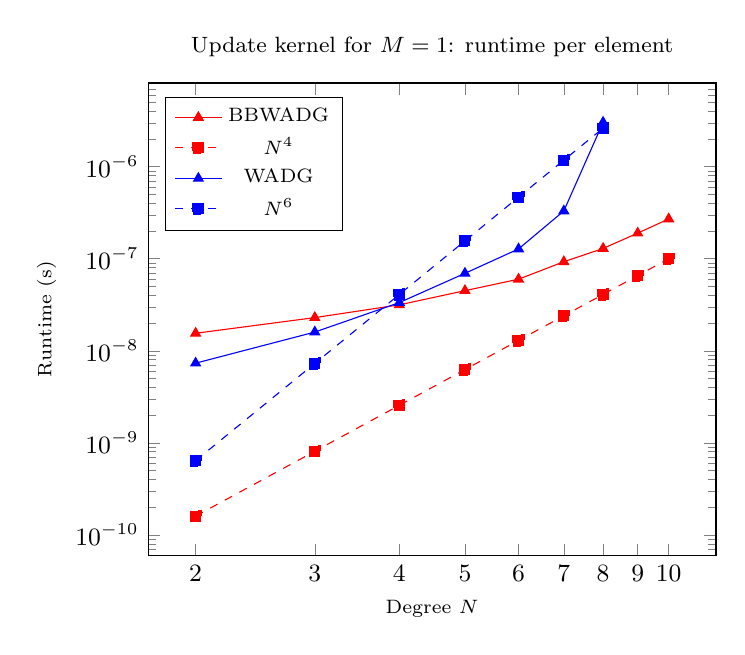
\begin{tikzpicture}
\begin{loglogaxis}[
width=.725\textwidth,
title = {Update kernel  for $M=1$: runtime per element },
xlabel=Degree $N$,
ylabel=Runtime (s),
xtick = data,
ticklabel style = {font=\small},
xticklabels={$2$,$3$,$4$,$5$,$6$,$7$,$8$,$9$,$10$},
legend style={font=\scriptsize},
legend pos = north west
]
\addplot[color=red,mark=triangle*] 
coordinates {
	(2,0.0000000154975 )
	(3,0.0000000229375)
	(4,0.0000000315594)
	(5,0.0000000449963)
	(6,0.0000000599558)
	(7,0.0000000927645)
	(8,0.000000129382)
	(9,0.000000189771)
	(10,0.000000270587)
};

\addplot[dashed, color=red,mark=square*] coordinates {
	(2,0.00000000016)
	(3,0.00000000081)
	(4,0.00000000256)
	(5,0.00000000625)
	(6,0.00000001296)
	(7,0.00000002401)
	(8,0.00000004096)
	(9,0.00000006561)
	(10,0.00000010000)
};


\addplot[color=blue,mark=triangle*] 
coordinates{(2,7.33677e-09)(3,1.5973e-08)(4,3.3419e-08)(5,6.9422e-08)(6,1.27759e-07)(7,3.30517e-07)(8,3.03384e-06)};
%coordinates {
%	(2,0.0000000101731 )
%	(3,0.0000000199103)
%	(4,0.0000000368739)
%	(5,0.0000000822495)
%	(6,0.000000242786)
%	(7,0.00000046937)
%	(8,0.00000289899)
%};

\addplot[dashed, color=blue,mark=square*] coordinates {
	(2,0.00000000064)
	(3,0.00000000729)
	(4,0.00000004096)
	(5,0.00000015625)
	(6,0.00000046656)
	(7,0.00000117649)
	(8,0.00000262144)
};
\legend{BBWADG,$N^4$, WADG,$N^6$}
\end{loglogaxis}
\end{tikzpicture}
\end{figure}

}

\frame{
\setcounter{subfigure}{0}
\frametitle{BBWADG: update kernel speedup over WADG (acoustics)}

\begin{table}
   \centering
   \begin{tabular}{|c||c|c|c|c|c|c|c|} % Column formatting, @{} suppresses leading/trailing space
 \hline
%& $N=2$ 
& $N=3$ & $N=4$ & $N=5$ & $N=6$ & $N=7$ & \textcolor{red}{$N=8$} \\
   \hline
%WADG  &  1.86e-8 &  3.74e-8  & 8.08e-8  & 2.34e-7 &   4.68e-7 &  2.90e-6\\
WADG  &          1.60e-8  &  3.34e-8 &   6.94e-8 &  1.28e-7 &  3.31e-7  &  \textcolor{red}{3.03e-6}\\
  \hline
BBWADG &   2.20e-8 &  3.30e-8 &   4.42e-8 &   6.01e-8 &  9.46e-8 & 1.31e-7 \\
  \hline
%Speedup & 0.85 &  1.13 & 1.83  & 3.90 & 4.95 & 22.2\\
Speedup &    0.7260 &    1.0127 &    1.5706 &    2.1258 &    3.4938 &   \textcolor{red}{23.1591}\\
  \hline
\end{tabular}  
\vspace{.5em} 
\caption*{For $N\geq 8$, quadrature (and WADG) becomes much more expensive.}
\end{table}
\vspace{-2em}
\begin{figure}
\centering
\subfloat[$N= 7$ quadrature]{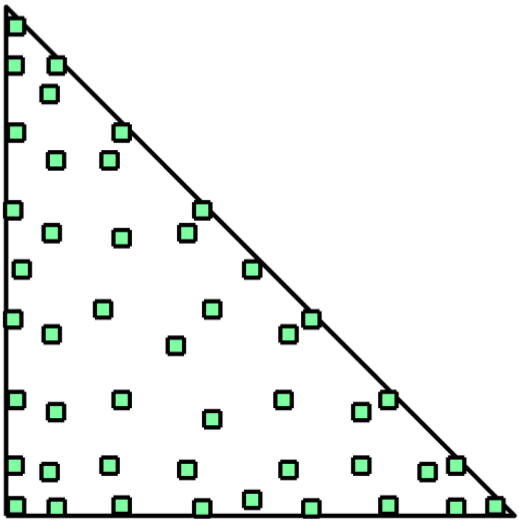
\includegraphics[width=.275\textwidth]{figs/quadrature_noTP.png}}
\hspace{2em}
\subfloat[$N =  8$ quadrature]{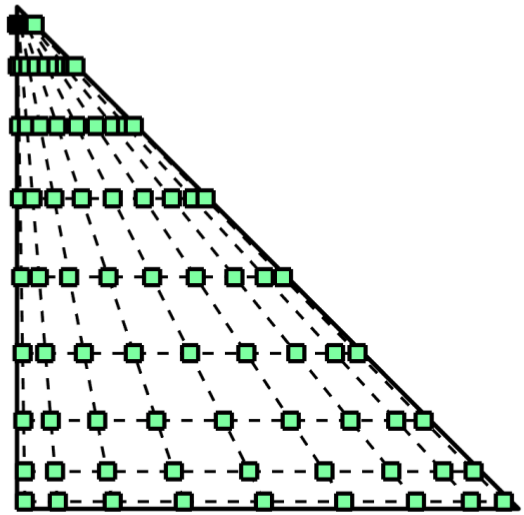
\includegraphics[width=.275\textwidth]{figs/quadrature_TP.png}}
%\caption*{For $N\geq 8$, WADG becomes much more expensive (more quadrature points).}
\end{figure}
}

\frame{
\frametitle{Summary and acknowledgements}

\vspace{1em}
\begin{itemize}
\item Weight-adjusted DG: stability and efficiency for heterogeneous media.
\vspace{.01em}
\item BBWADG: improved complexity for approximate wavespeeds.
\vspace{1em}
\item This work is supported by the National Science Foundation under DMS-1712639 and DMS-1719818. 
\end{itemize}
\vspace{.25em}
\begin{center}
Thank you!  Questions?
\vspace{.5em}

{
\includegraphics[width=.15\textwidth]{figs/nsf.jpg}}
\end{center}


\let\thefootnote\relax\footnotetext{\tiny Chan, Hewett, Warburton.\ 2016.  {Weight-adjusted DG methods: wave propagation in heterogeneous media} (SISC).}
\let\thefootnote\relax\footnotetext{\tiny Chan 2017.  Weight-adjusted DG methods: matrix-valued weights and elastic wave prop.\ in heterogeneous media (IJNME).}
\let\thefootnote\relax\footnotetext{\tiny Chan, Warburton 2015.  {GPU-accelerated Bernstein-Bezier discontinuous Galerkin methods for wave propagation} (SISC).}
}

%\frame{
%\begin{center}
%The authors thank TOTAL E\&P Research and Technology USA\\
%for their generous support of this work.
%\end{center}
%\let\thefootnote\relax\footnotetext{\tiny Chan, Warburton 2015. {GPU-accelerated Bernstein-Bezier DG methods for wave problems}.}
%\let\thefootnote\relax\footnotetext{\tiny Chan, Warburton 2015.  A short note on a Bernstein-Bezier basis for the pyramid.  (SISC, accepted)}
%\let\thefootnote\relax\footnotetext{\tiny Chan, et al.\ 2016.  {WADG methods I: wave propagation in heterogeneous media}.  In preparation.}
%\let\thefootnote\relax\footnotetext{\tiny Chan, et al.\ 2016.  {WADG methods II: curvilinear meshes}.  In preparation.}
%}
%% =================== extra slides =======================

%\begin{frame}[noframenumbering]
%\frametitle{Additional slides }
%
%\end{frame}


\bibliographystyle{plain}
{\scriptsize
\bibliography{pyramids}
}

\end{document}
